\documentclass[12pt,a4paper]{report}

\usepackage[utf8]{inputenc}
\usepackage[T1]{fontenc}
\usepackage{mathptmx}
\usepackage{pifont}
\usepackage{amsmath}
\usepackage{graphicx}
\usepackage{hyperref}
\usepackage{xcolor}
\usepackage{listings}
\usepackage{tocbibind}
\usepackage{pdfpages}
\usepackage{booktabs}
\usepackage{makecell}
\usepackage{subcaption}
\usepackage{fancyhdr}
\usepackage{float}
\usepackage{titlesec}
\usepackage{sectsty}
\usepackage{tocloft}
\usepackage{lipsum}

\hypersetup{
colorlinks=true,
urlcolor=blue,
linkcolor=black
}

\pagestyle{fancy}
\fancyhf{}
\fancyhead{\nouppercase{\rightmark\hfill\leftmark}}
\fancyfoot[L,R]{\hfill\thepage\hfill}
\setlength{\headheight}{15pt}
\titleformat{\chapter}[display]{\normalfont\Large\bfseries}{Chapter \thechapter}{20pt}{\uppercase}
\setlength{\cftchapnumwidth}{2.2cm}
\setlength{\cftfignumwidth}{2.2cm}
\setlength{\cfttabnumwidth}{2.2cm}
\renewcommand{\cftchappresnum}{Chapter }
\renewcommand{\cftfigpresnum}{Figure }
\renewcommand{\cfttabpresnum}{Table }
\renewcommand{\figurename}{FIGURE}
\renewcommand{\tablename}{TABLE}
\renewcommand{\contentsname}{Table of Contents}
\renewcommand{\abstractname}{General Introduction}

\begin{document}

\includepdf[pages={3,1}]{./pdfs/Page Garde Rapport Stage(Ang) 2.pdf}

\chapter*{Acknowledgements}
\addcontentsline{toc}{chapter}{Acknowledgements}
\par It is with a great pleasure that I reserve these lines to express my heartfelt gratitude, indebtedness, and appreciation to everyone who has ever contributed to the fulfillment of this internship, either directly or indirectly.\newline
\par First and foremost, I would like to express my gratitude to my corporate internship supervisor, Mr. Hazem RAOUAFI who is a Software and Cloud Engineer at Standard Sharing Software, for playing a major role in the successful completion of this project. His constant assistance throughout the duration of my internship has greatly contributed to its success and helped to broaden my perspectives on ways to improve the project.
\bigskip\newline I would also like to thank my academic supervisor, Mrs. Chifaa GHANMI, who guided and encouraged me while also providing valuable advice along the way, and for her patience and incessant support during the internship period.
\bigskip\newline Likewise, I would like to express my recognition and appreciation to all the teachers at ESPRIT, for their diligence and enthusiasm to provide the highest quality of training and education over the years of studies.
\bigskip\newline Also, I want to express my dearest gratefulness to my parents in particular, no dedication can express my sincere feelings for their unlimited patience, their encouragement, and for their great sacrifices, as well as all the members of my close family and friends.
\bigskip\newline Finally, I would like to extend my thankfulness and respect to the members of the jury for their expertise and meticulous review of this report, hoping it clearly and thoroughly reflects the achieved work.

\tableofcontents

\listoffigures
\listoftables

\chapter*{Glossary}
\markboth{Glossary}{Glossary}
\addcontentsline{toc}{chapter}{Glossary}
\begin{itemize}
    \item \textbf{3S} : Standard Sharing Software (The hosting company)
    \item \textbf{RAG} : Retrieval-Augmented Generation
    \item \textbf{LLM} : Large Language Model
    \item \textbf{EKB} : Entreprise Knowledge Base
    \item \textbf{AI} : Artificial Intelligence
    \item \textbf{GPT} : Generative Pre-trained Transformer
    \item \textbf{NLP} : Natural Language Processing
    \item \textbf{RL} : Reinforcement Learning
    \item \textbf{RLHF} : Reinforcement Learning from Human Feedback
    \item \textbf{SBERT} : Sentence Bidirectional Encoder Representations from Transformers (or Sentence Transformers for short)
    \item \textbf{HF} : Hugging Face
    \item \textbf{MTEB} : Massive Text Embedding Benchmark
    \item \textbf{ML} : Machine Learning
    \item \textbf{DL} : Deep Learning
    \item \textbf{URL} : Uniform Resource Locator
    \item \textbf{API} : Application Programming Interface
    \item \textbf{OS} : Operating System
    \item \textbf{CPU} : Central Processing Unit
    \item \textbf{GPU} : Graphics Processing Unit
    \item \textbf{RAM} : Random-access memory
    \item \textbf{DB} : Database
    \item \textbf{CUDA} : Compute Unified Device Architecture
    \item \textbf{VM} : Virtual Machine
    \item \textbf{WSL} : Windows Subsystem for Linux
    \item \textbf{JS} : JavaScript
    \item \textbf{HTML} : Hypertext Markup Language
    \item \textbf{a.k.a.} : also known as
    \item \textbf{e.g.} : for example
    \item \textbf{i.e.} : that is
\end{itemize}

\begin{abstract}
    \addcontentsline{toc}{chapter}{General Introduction}
    \par With the recent progress in technology and Artificial Intelligence in particular, businesses became increasingly interested in leveraging the domains of application of these advancements in order to optimize their internal processes and the efficiency and productivity of their employees. The emergence of Generative AI chatbots (e.g., ChatGPT, Google Gemini, etc...) has opened up exciting new perspectives in this domain; It came up with an alternative approach for searching large volumes of information, delivering significantly more insightful results in less time and effort than traditional methods.\medskip
    \par This report presents the design and implementation of an Entreprise Knowledge Base searching tool to facilitate the quick and precise retrieval of custom and proprietary information by employees, thereby enhancing knowledge-intensive workflows.
    This solution was conceived in fulfillment of an end-of-studies internship project at "Standard Sharing Software", specifically tailored to the company's requirements. It provides users with functionalities to augment and organize the knowledge base, enabling them to retrieve the most relevant contents thereof when needed.\smallskip
    \par To fulfill the purposes of this solution, various technologies have been explored and implemented: A Vector Store for persisting documents into the knowledge base, embeddings and similarity search algorithms for retrieving the most relevant passages corresponding to user queries, Large Language Models (LLMs) to synthesize these retrieved passages, condensing them into concise and understandable responses and Prompt Engineering for the optimal utilization of LLMs' capabilities, among other techniques. The synergistic orchestration of these diverse tools constitutes the Retrieval-augmented Generation (RAG) framework.\medskip
    \par This report first details the context and the compelling need for such a solution within the company. It then presents the conception phase of the project, highlighting the functional and non-functional requirements along with the general use case diagram and planning out tasks and deadlines. It subsequently introduces the various technical terms employed throughout the project, elucidating the rationale behind the selection and application of these technologies. Finally, it concludes by detailing the implementation process and the achieved results, while also acknowledging potential limitations and avenues for further improvement.\bigskip
    \par\textit{\textbf{Keywords:} Retrieval-augmented Generation (RAG), Large Language Models (LLMs), Generative AI, Vector Store, Embeddings, Similarity Search, Prompt Engineering}
\end{abstract}

\chapter{Project Framework}

\section{Introduction}
This chapter presents a general overview of this end-of-studies project. It lays out the context and influences which made it relevant in current settings.
First, it describes the background and sequence of developments that brought much of the employed technologies into existence. Next, it introduces the hosting company and discusses its necessity for such a novel solution. And finally, it lists the pursued objectives and innovations which address the insufficiencies of existing solutions.

\section{Background}
Business Knowledge is both integral and proprietary for any enterprise. The contents of private documents are useful for internal employees who are constantly consuming it to accomplish their workstreams. It becomes evident when considering that modern software development and network infrastructure deployment (among many other fields) are often based on exploring exhaustive documentation and lengthy research papers. Paradoxically, this upfront research and learning introduce a sort of bottleneck, requiring much time before a new project gets initiated. In most cases, a further looking up for previously reviewed information is often required. Accelerating delivery, however, remains a key aspiration for organizations seeking a competitive edge. This together emphasizes the need to consider and propose innovative solutions which would help reduce the preliminary requirements and achieve faster delivery cycles.\medskip\newline
In line with this discussion, it is worth highlighting the evolving landscape of web search in the contemporary era. We used to input a query into a search engine (e.g. Google) and it would look through its indexed webpages and then return a list of the most relevant pages which we would then read until we have a satisfying answer. This paradigm has veered towards generative AI chatbot solutions, like ChatGPT, Copilot and Gemini, which leverage Machine Learning algorithms to mimic the natural language understanding capability of humans to generate short and accurate answers based on public information and the open web.\smallskip\newline
Auspiciously, the underlying technology that empower this kind of chatbots is discrete from their corresponding platforms, i.e., it can be integrated in other projects as a library or a software component rather than being exclusive to their native applications, which makes customizing their functioning and augmenting their knowledge possible. This presents an interesting theme for an internship project which attempts to build upon these technologies to provide a much needed solution for an entreprise with many activities and projects to accomplish and for a data science student aspiring to continuously learn the newest trends in AI and Machine Learning.

\section{Hosting Company}
The hosting of this project was managed by Standard Sharing Software (3S).
\smallskip\newline
\begin{figure}[H]
    \centering
    
\includegraphics[width=0.4\linewidth]{./figures/logo_3S.png}
    \caption{Standard Sharing Software logo}
\end{figure}
3S Group, founded in 1988 with the mission of transforming the Tunisian technological landscape, is a leading company in Tunisia specializing in the integration of IT infrastructures and the provisioning of advanced technological solutions. The group brings together more than 650 employees spread across 16 separate affiliates, each specialized in different cutting-edge technologies, covering a wide range of sectors including the integration of IT infrastructures, the provisioning of internet services, the edition of ERP solutions, and the management of multichannel call centers.\newline
It is based in Montplaisir, Tunis, Tunisia (headquarters), and in Charguia 1, Tunis (the office where this internship was conducted), with different teams specializing in Network and Telecommunication infrastructures, Cyber security, Cloud Computing and Software. This project was organized and executed in the Cloud and Software department of the company yet close collaboration with these different units was required since they constitute the target users of this project.\newline
3S Group's work culture helped the success of this project with its core values of commitment, excellence, innovation and teamwork, which were reflected during the whole duration of this internship, from project initialization until delivery, as evidenced by the organizers's relentless dedication to meeting project deadlines, the pursuit of using innovative tools, the collaborative problem-solving approach, and the unwavering commitment to delivering exceptional results.

\section{Study of the Existing}
\subsection{Problem Statement}
Traditional enterprise search engines, including those currently utilized by 3S employees, face significant limitations in effectively comprehending the context of user queries and the nuances of human language. These systems often rely on exact text matching, which fails to capture the semantic meaning behind queries, leading to inefficient and incomplete retrieval of information. Even with the advent of AI tools that enhance Natural Language Processing (NLP), accessing and leveraging large volumes of enterprise data remains a formidable challenge for proprietary systems.

The complexity is further compounded by increasing regulatory scrutiny on AI products, driven by concerns over privacy and copyright infringement. While such regulations are essential for protecting sensitive information and ensuring compliance with legal standards, they also pose obstacles to integrating advanced AI tools into enterprise environments. This underscores the need for companies to develop their own tailored solutions to fully harness recent AI advancements while navigating regulatory constraints.

A Retrieval-Augmented Generation (RAG) system addresses these challenges by combining state-of-the-art retrieval techniques with large language models (LLMs). This system enhances employees' access to enterprise data by accurately locating relevant information from vast datasets and presenting it in a coherent, contextually appropriate manner. Ultimately, this approach empowers employees to make better-informed decisions, boosts productivity, and ensures compliance with privacy and copyright standards.
\subsection{Criticism of the Existing}
In the table below, an identification and comparison between a few existing solutions has been undertaken to understand their limitations and how to build upon them.
\begin{table}[H]
    \centering
    \begin{tabular}{|c|c|c|c|}
        \toprule
        \textcolor{darkgray}{\textbf{\makecell{Solution}}}  & \textbf{\makecell{LLM                                                                                               \\Chatbots}}                                     & \textbf{\makecell{NotebookLM}}                                       & \textbf{\makecell{Verba}}                                             \\
        \midrule
        \textcolor{darkgray}{\textbf{\makecell{Developer}}} & \makecell{Google, OpenAI                                                                                            \\and Microsoft}                                 & Google                                                    & Weaviate                                                   \\
        \midrule
        \textcolor{darkgray}{\textbf{\makecell{RAG-based                                                                                                                          \\ (with persistent storage)}}} & \textcolor{red}{\ding{56}}        & \textcolor{green}{\ding{52}}                                & \textcolor{green}{\ding{52}}  / \textcolor{red}{\ding{56}} \\
        \midrule
        \textcolor{darkgray}{\textbf{\makecell{Enterprise                                                                                                                         \\focused}}} & \textcolor{red}{\ding{56}}                                & \textcolor{red}{\ding{56}}                                & \textcolor{green}{\ding{52}}  / \textcolor{red}{\ding{56}} \\
        \midrule
        \textcolor{darkgray}{\textbf{Extensible}}           & \textcolor{green}{\ding{52}} / \textcolor{red}{\ding{56}} & \textcolor{red}{\ding{56}} & \textcolor{red}{\ding{56}} \\
        \midrule
        \textcolor{darkgray}{\textbf{\makecell{Multiple                                                                                                                           \\LLMs}}}      & \textcolor{red}{\ding{56}}                                & \textcolor{red}{\ding{56}}                                & \textcolor{green}{\ding{52}}                               \\
        \midrule
        \textcolor{darkgray}{\textbf{\makecell{User-LLM                                                                                                                           \\feedback}}}  & \textcolor{green}{\ding{52}} & \textcolor{red}{\ding{56}} / \textcolor{green}{\ding{52}} & \textcolor{red}{\ding{56}}                                 \\
        \midrule
        \textcolor{darkgray}{\textbf{\makecell{Stable                                                                                                                             \\ (Not experimental)}}} & \textcolor{green}{\ding{52}} & \textcolor{red}{\ding{56}}                                & \textcolor{red}{\ding{56}}                                 \\
        \bottomrule
    \end{tabular}
    \caption{Comparison of existing solutions}
    \begin{flushleft}
        \par The table above provides a comparative review of some of the most suitable similar solutions (AI chatbots, NotebookLM, and Verba), highlighting their features and limitations.\newline "RAG-based" refers to whether or not the solution automatically retrieves relevant passages from a knowledge base, rather than passing the context manually each time. "Entreprise focused" suggests that the solution was designed to address entreprise requirements such as managing and sharing different knowledge base partitions for different teams. "Extensible" means that the solution can be further tweaked or developed to modify and add new features. "Multiple LLMs" indicates that the solution provides multiple models generating responses each time. "User-LLM feedback" signifies the ability for users to provide feedback for generated responses, which can be used to enhance future behavior. "Stable" refers to stability of the product.
    \end{flushleft}
\end{table}
In general, one can utilize any ready-to-use LLM-powered chatbot (e.g. ChatGPT, Microsoft Copilot, Google Gemini, and many others). But these solutions, even though allowing document-answering, don't come with document persistence, which means by leaving the chat, the documents are gone unless re-uploaded.\newline
Google is currently experimenting with a new solution (NotebookLM) which allows exactly that by connecting to cloud-hosted documents, in addition to methods allowing to upload local files and webpage content from URLs. Nonetheless, this falls short for enterprise usage as it is intended for casual use cases (e.g. note taking, document editing suggestions and personal project research) rather than question-answering from a large knowledge base and does not provide features to share documents between different users. On the other hand, Weaviate, a company behind a vector store implementation, maintains \href{https://github.com/weaviate/Verba}{a repository on GitHub} which addresses the same objectives as this project. Their solution, called Verba, is a well-organized open-source project that can be easily deployed on-premises or in a cloud environment. However, several challenges need to be addressed before a company can use and adapt it to their specific needs: customization is difficult, if not impossible, given that the project depends on many packages they developed or contributed to (goldenverba, weaviate, ...), requiring many API keys from various providers (vector database, LLMs, cloud providers, etc...), in addition to the inability to create and manage different databases for different teams.\smallskip\newline
This scarcity and inadequacy of available solutions raises the need to design and develop a custom product suitable for the specific needs and requirements set up by individual enterprises, which are discussed in the following section for our case.

\section{Proposed Solution}
This project aims to develop a novel search functionality that leverages retrieval-augmented generation techniques to deliver insightful results for enterprise data, by addressing general-purpose large language models' limitations, which can be summed up in data confinement to training phase and private data access. The system will prioritize the following objectives.
\subsection{Objectives}
\begin{itemize}
    \item Enhance AI-generated responses with External Knowledge: Retrieve relevant passages from a curated enterprise knowledge base each time a LLM is prompted to improve its factual grounding and reduce the risk of hallucinating.
    \item Flexible Data Ingestion and Organization: Implement diverse methods for multi-source, format-agnostic file content and document indexing into manageable and domain-specific vector databases to tailor to enterprise needs and potential evolution.
    \item Diverse Answering Options: Allow the selection from a list of various Large Language Models for answering and just-in-time (of generating responses) data scraping to diversify and improve results each time.
    \item User-Driven Feedback: Integrate a mechanism for providing user feedback for LLM-generated responses which can be used to rank future results and further train and improve LLMs (when supported).
    \item Leverage RAG-based metrics for evaluation: Employ retrieval-augmented generation evaluation metrics to assess the quality of pipeline stages' results (retrieval quality/accuracy, context-generation consistency, answer relevancy)
\end{itemize}
\subsection{Significance of RAG}
RAG technology comes with many benefits for businesses in the context of leveraging generative AI models for content searching:
\begin{itemize}
    \item Private and up-to-date data: Even with the best performing generative AI chatbots, it is challenging to maintain relevancy in an enterprise environment. By allowing AI models to connect to external knowledge bases and personal data, much more relevant results can be achieved.
    \item Cost-effective: Even with the availability of open-source LLMs and cloud-based FMs (Foundational Models), the computational and financial costs of re-training such models on domain-specific or private data can be high. By circumventing the re-training phase of LLMs, a huge gain can be brought off using this technique.
    \item More control and customization: It is easy for developers to customize RAG pipelines: Adapting to changing requirements and sources of information, troubleshooting model performance and results, restricting access to some information for authorized users, etc...
    \item User trust: By enabling user choices and interference in the overall process of RAG, users can look up how their choices in information sources and LLM selections directly affect the system's performance and results.
\end{itemize}
In many ways, RAG techniques, when combined with an effective Prompt Engineering approach, provide an alternative framework to re-training or fine-tuning with better adaptability and performance on knowledge-intensive tasks. This is because it is difficult for LLMs to capture new factual information through unsupervised fine-tuning. The following figure demonstrates the effectiveness of a RAG pipeline when a model does not have access to recent information.
\begin{figure}[H]
    \centering
    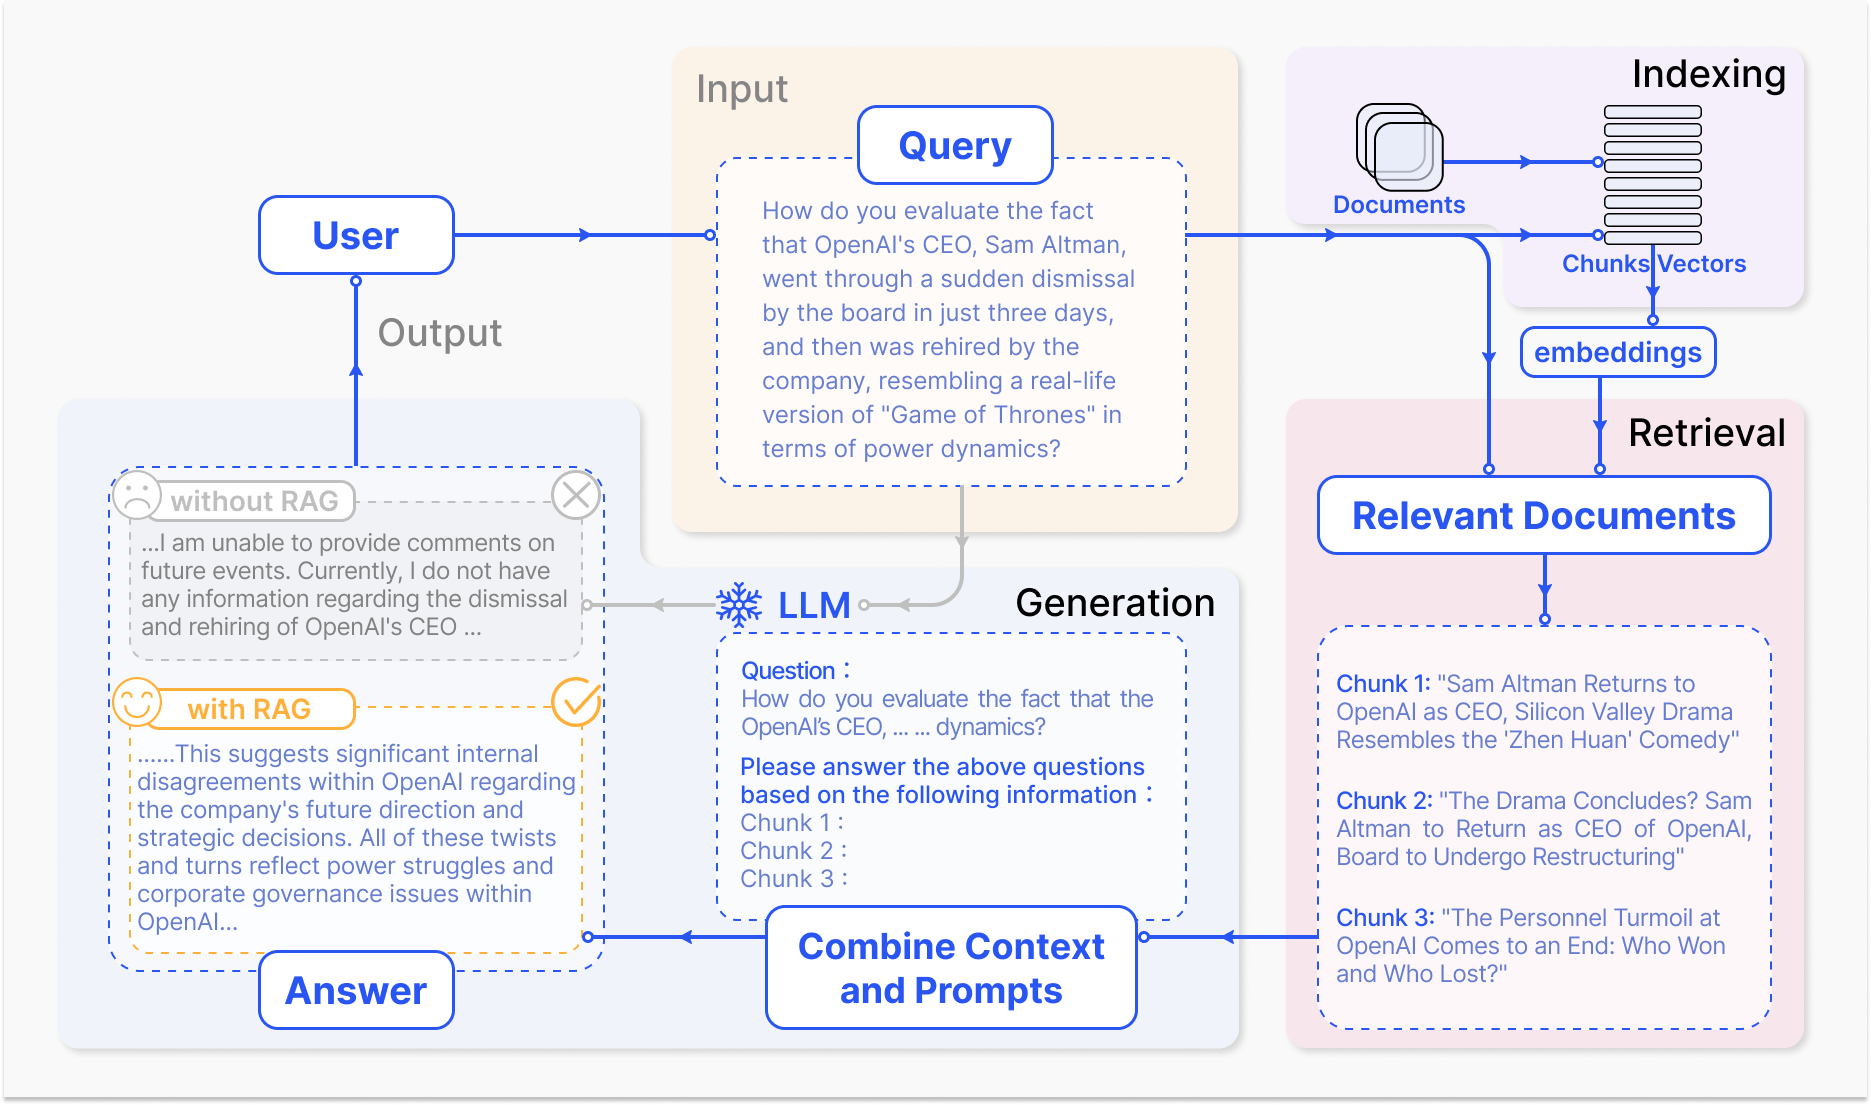
\includegraphics[width=\linewidth]{./figures/RAG_case.png}
    \caption{An illustration of a RAG pipeline in work. (\href{https://arxiv.org/html/2312.10997v5}{[Retrieval-Augmented Generation for Large Language Models: A Survey]}, March 2024)}
    \begin{flushleft}
        \small A comparative representation between a simple LLM and a RAG process applied to question answering. Prompting the LLM directly resulted in its inability to provide a suitable answer because its does not have access to new information. The RAG process, on the other hand, has successfully identified the relevant information from the knowledge base and made the LLM capable of generating a factual response.
    \end{flushleft}
\end{figure}
\subsection{Significance of the Solution}
The proposed Generative AI solution would help employees find answers from enterprise knowledge without having to browse vast amounts of documents. This is enabled by augmenting LLM knowledge using the techniques of retrieval-augmented generation and prompt engineering for context precision. It would also allow them to interfere in the steps of answer-generation by providing ways to customize the external knowledge base and conduct online researching, powered by traditional search engines and generative AI researching tools, through a unified interface.\medskip\newline
From an educational perspective, this project presents a valuable opportunity to gain expertise on some of the most capable ML models and personalize and extend their functioning. The anticipated learning outcomes of accomplishing this project include an enhanced perception of large models' parameters and how they affect performance, picking up prompt engineering techniques, planning out and implementing RAG pipelines that tailor to complex requirements, using both local and cloud components, in addition to developing various data scraping methods.

\section{Conclusion}
This first chapter has given grounds for the development of the proposed solution for the hosting company, by presenting the limitations of existing solutions and identifying key objectives to implement during the internship.\newline
In the following chapter, we will break down the project's requirements and select a management strategy, in addition to identifying tasks and setting up deadlines.

\chapter{Project Scope and Planning}

\section{Introduction}
This chapter is dedicated to a comprehensive analysis of system requirements, encompassing both functional and non-functional attributes necessary to meet our user needs. Subsequently, a suitable project management methodology will be selected to finally outline a project plan, including task delineation and associated deadlines.

\section{Project Requirements}
In this section, we outline the comprehensive requirements for the project, essential for breaking down the project goals into tasks and guiding development efforts.\newline
First, we start by outlining the main actors involved in the system's functioning.
\subsection{Actors Identification}
An actor is an abstract representation of an entity which interacts with the system being conceived. This element can be a user, a group of users, or an external system, which trigger the system's processes.\newline
The actors are categorized as follows:
\begin{itemize}
    \item \textbf{Regular User:} This role represents an employee who has access to use the application, which provides them with answers to their questions based on content stored in vector databases.
    \item \textbf{Database Manager:} A DB manager is a regular user that has access to authentication keys for a database. In addition to the regular features which a normal user has access to, this role allows them to access and index new content into a shared database.
    \item \textbf{Administrator:} The role of the application administrator is to manage the default configuration and parameters of the application.
\end{itemize}
\subsection{Functional Requirements}
After identifying the different actors of the system, we will describe the features which will be integrated in the system and assign them to these roles.
\subsubsection{Regular User}
\begin{itemize}
    \item \textbf{Response source choice:} The system should allow users to pick the vector databases from which information relevant to their queries will be retrieved.
    \item \textbf{Data augmentation:} The system should provide external knowledge feteching methods to allow the ingestion of related information from real-time sources.
    \item \textbf{Translation:} The system should enforce cross language capabilities for accurate and consistent behavior in a multilingual context.
    \item \textbf{Model Selection:} The system must integrate different Generative AI models from which a user can select options relative to the API they have access to.
    \item \textbf{Answers:} The system must be able to process user queries, retrieving relevant information from the selected databases and generating answers based on users choices, and then prioritize the more informative responses.
    \item \textbf{Feedback options:} The system should allow users to give their feedback for each response result, and use this feedback when ranking further answers.
\end{itemize}
\subsubsection{Database Manager}
\begin{itemize}
    \item \textbf{Database authentication:} The system should allow users to gain database management access with a DB name and passphrase.
    \item \textbf{Database management:} The system must allow DB managers to access the DB content and index new information into it.
\end{itemize}
\subsubsection{Application Administrator}
\begin{itemize}
    \item \textbf{Configuration management:} The system should provide options for the Administrator to change the default configuration: API keys, initial databases with names and passphrases for different teams, and changing the directory for storing application data and cache.
\end{itemize}
\subsection{Non-function Requirements}
In addition to the functionalities that the application must provide for its users, there are other characteristics and attributes which the project must respect and pursue. These constraints do not describe the services made available for the end user, but rather focus on their quality and performance.
\begin{itemize}
    \item \textbf{Performance:} The time it takes for Loading, using and navigating pages of the app should be minimal, even in the case of multiple simultaneous connections.
    \item \textbf{Conviviality and Usability:} The interfaces should be intuitive and accessible.
    \item \textbf{Maintainability:} The source code should be organized to allow the improvement and evolution of the project.
\end{itemize}

\section{Project Management}
Upon establishing the project's requirements and functionalities, it is now time to plan out expected tasks into an organized timetable. This section of the chapter addresses that. It is composed of two parts, one explaining the suitability of the employed methodology throughout the project, and another detailing the tasks to be undertaken.
\subsection{Methodology}
Given the nature of this project, the Scrum methodology was selected for the implementation of the system. This iterative approach allowed for the continuous development and refinement of tasks (Sprints) throughout this internship by allowing users' interference and feedback during the development process. This flexibility was particularly valuable in this end-of-studies project where the final requirements kept evolving.
\begin{figure}[H]
    \centering
    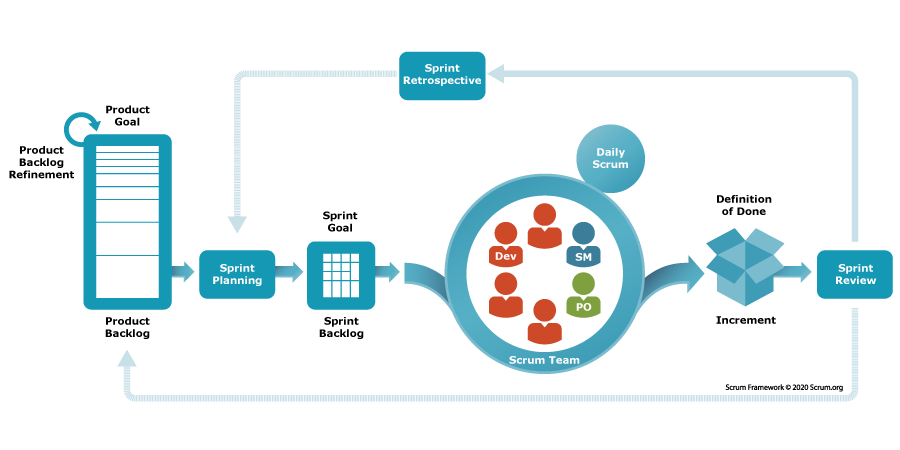
\includegraphics[width=\linewidth]{./figures/scrum-framework-9.29.23.png}
    \caption{Scrum framework \href{https://www.scrum.org/resources/what-scrum-module}{[What is Scrum (scrum.org)]}}.
\end{figure}
This methodology defines the steps to implement a project as follows :
\begin{enumerate}
    \item Project Planning : Defining the project's overall objectives and values to be gained by users. And on a smaller scale, the specific Sprint objectives.
    \item Product Backlog : Identifying and re-prioritizing the customer's requirements into an organized list of Sprints.
    \item Sprints : Identifying and organizing tasks into a list of Sprints
    \item Scrum Meetings : Daily short meetings to discuss progress and challenges to complete a Sprint's tasks.
    \item Increment development : Iteratively complete Sprint cycles (planning, design, coding, testing and review) to complete increments.
    \item Sprint Review : Review of the completed work with the entreprise supervisor
    \item Sprint Retrospective : Discussing what went good and what went bad during the Sprint to gain better insight on what can be improved in the future.
\end{enumerate}
The following section demonstrates the influence of this agile methodology, by showcasing a planned timetable in compliance with the iterative approach of the Scrum methodology.
\subsection{Planning}
To plan out the implementation of user requirements, we divided and organized the user requirements into a list of tasks and increments in accordance with the agile methodology.
The following Gantt Chart illustrates the timetable of planned tasks and how they were split into smaller chunks to accomplish them and iterate the development process over different time segments.
\begin{figure}[H]
    \centering
    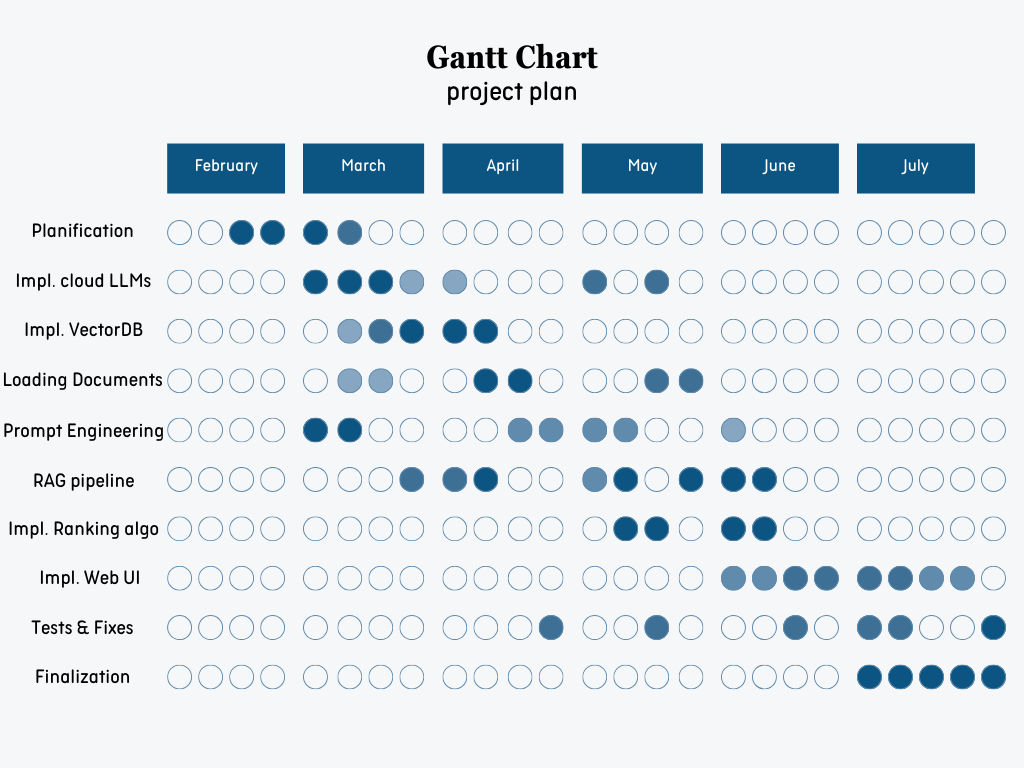
\includegraphics[width=\linewidth]{./figures/gantt-chart-1.png}
    \caption{The planned Gantt Chart}
\end{figure}
\begin{flushleft}
    \par This method allowed to accomplish Increments, which represent tangible steps towards the final project implementation: The first iteration (second week of March) was planned to implement Large Language Models standalone answering functionality (without RAG or a vector store), combining cloud-based LLMs with prompt engineering techniques. The next iteration focused on initiating the RAG pipeline by implementing a vector store index with static content, modifying Prompts to control the LLMs' factual grounding, after which some testing and further development was conducted to tailor to the different LLMs and make the vector store more dynamic by implementing data augmentation methods. After these two iterations which were completed by the start of May, further enhancement was undertaken to customize the indexing methods to tailor to different teams and the retrieval phase to minimize dissimilar results, in addition to supplying more data augmentation knowledge sources through APIs and the exploration of how a ranking algorithm could be implemented. The final iteration focused on integrating all the functionalities into a web interface, implementing a user feedback option and enhance answer ranking and validating the results with the corporate supervisor.
\end{flushleft}

\section{Conclusion}
This chapter, along with the previous one, clarified the project's roadmap and helped breaking down the problem statement into a list of tasks to be implemented. These tasks are now explained in more detail in the following chapter, which discusses the implementation phase of this project.

\chapter{Technical Foundations}

\section{Introduction}
For the purpose of this project, an extensive investigative study into Retrieval-augmented Generation process has been conducted. This chapter explains RAG in more detail, explores its paradigms, outlines its components and provides the rationale behind the selection of certain choices.

\section{RAG Overview}
Retrieval-augmented Generation, or RAG for short, is an information retrieval pipeline consisting of mainly two consecutive processes: Retrieval and Generation.
\begin{itemize}
    \item The purpose of the first phase (retrieval) is to fetch, from a knowledge base containing a large number of documents, the passages that are most relevant to a given query. It gets initiated when a user submits a question to the system, and depending on the indexing method of the knowledge, calculates and determines a collection of short text paragraphs containing relevant data. This information constitutes the "context" in RAG glossary, and gets then passed to the next phase along with the input question.
    \item The second phase focuses on generating a suitable response for a given query. It achieves this by first structuring an instruction, composed of the question and context from the previous phase, in a format interpretable by a generative AI model. The model then analyses the instruction (or prompt) and based on its architecture, attempts to generate a suitable response.
\end{itemize}
The RAG technique represents a method for customizing the interaction with a generative AI model, and enables to control the referenced information in the generation process. In the next section, we explore some approaches to designing the overall pipeline and how to tailor its processes for more accurate results and better performance.

\section{RAG Paradigms}
The RAG process has significantly improved on the limitations of generative AI models by augmenting their knowledge while eliminating the need to re-train them. Even so, a simple RAG pipeline can still exhibit various flaws, such as retrieval-echoing generation, which means responding with the contents of the retrieved documents rather than adding more insights through the Generative AI models' capabilities. Moreover, this baseline RAG can still introduce hallucinations by confining the generative process to the retrieved documents, which may not be pertinent to the query in every occasion, such as in case where relevant information are not present or cannot be retrieved from the knowledge base. In this respect, as more research and engineering is continually being conducted, advanced spinoffs of RAG has emerged to reduce the mis-reckoning and limitations of simplistic RAG.
\begin{figure}[H]
    \centering
    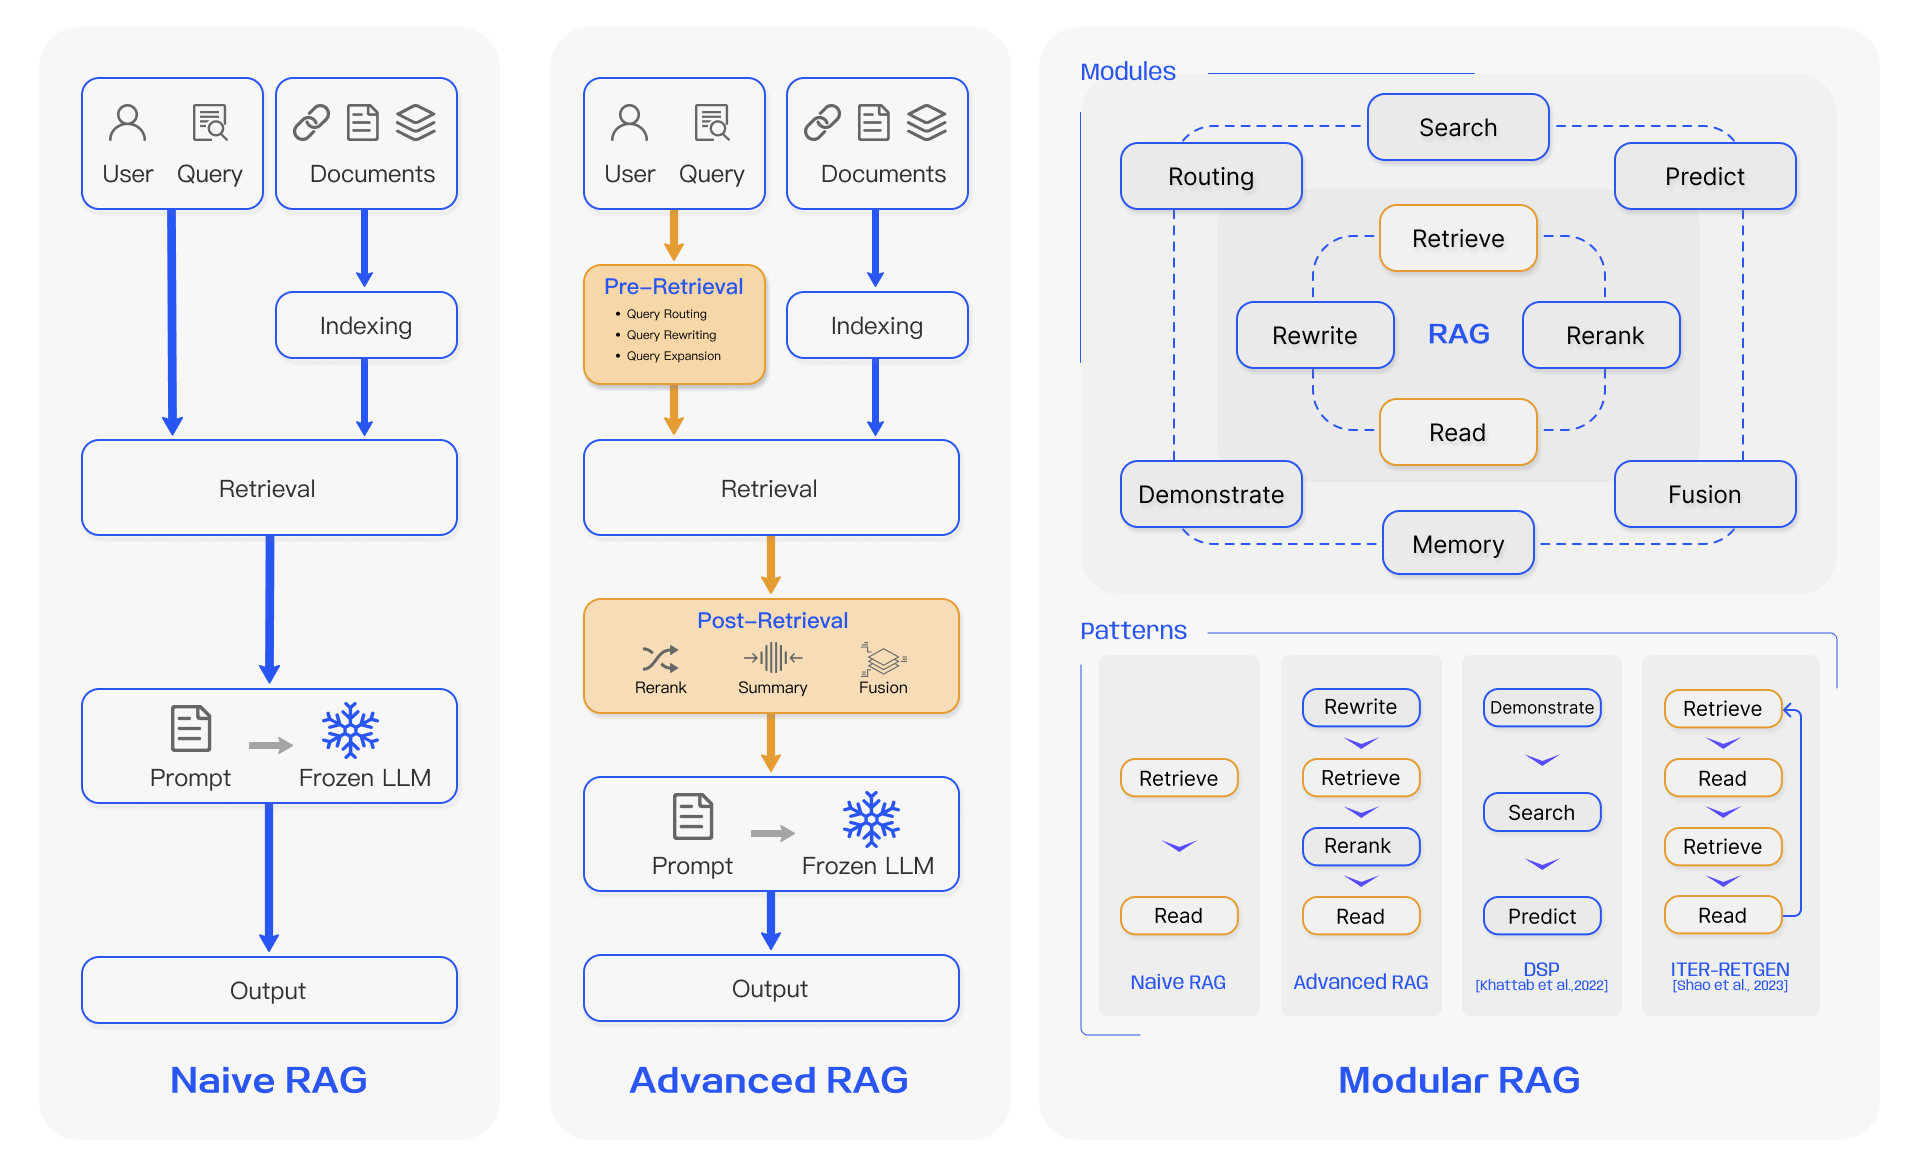
\includegraphics[width=\linewidth]{./figures/RAG_FrameCompre_eng.png}
    \caption{Comparison between the three paradigms of RAG: Naive, Advanced and Modular RAG \cite{ragforllmsasurvey}}
    \begin{flushleft}
        \small Naive RAG (LEFT)  mainly consists of three parts: indexing, retrieval and generation. Advanced RAG (MIDDLE) proposes multiple optimization strategies around pre-retrieval and post-retrieval, with a process similar to the Naive RAG, still following a chain-like structure. Modular RAG (RIGHT) is not limited to sequential retrieval and generation; it includes methods such as iterative and adaptive retrieval.
    \end{flushleft}
\end{figure}
In the light of this, we focus on the advanced RAG pipeline structure, which addresses many of the shortcomings of a naive RAG chain without introducing too much complexity to the overall pipeline, which results in very long question-to-generation delays and expensive API calls.
This paradigm involves knowledge base augmentation by routing the input query to other processes and external knowledge sources such as web content searching and generative research conducting, translating text across languages, context summarization and re-ranking, and LLM instructing through prompt engineering in addition to the evaluation and re-ranking of the generation phase' results. This is achieved through the introduction of two additional steps or processes into the overall pipeline: pre-retrieval and post-retrieval. The pre-retrieval phase focuses on selecting knowledge sources from which the context can be retrieved (query routing), translating the question if needed (query rewriting) and connecting it to external knowledge sources e.g. search engines and AI research generator (query expansion). The post-retrieval phase focuses on constructing the best prompt by interpolating and prioritizing more relevant context into it while eliminating unrelated parts. This phase also addresses content overload by filtering recurrent and repetitive information, compressing or summarizing context, and finally, as a post-generation step, re-ranking generated answers (in our case of multiple LLMs). These extra steps would result in better user experience in case knowledge base augmentation is required just-in-time of answer-generation or a re-ranking/adjustment of either retrieval or generation phase output is required.\bigskip\newline
Having highlighted the mains steps of the RAG pipeline, it is now worth examining the different components that needs to be integrated in the system and the interaction between them, which will be discussed in the next section.

\section{System Architecture}
The different processes and subprocesses which a RAG pipeline involves require a number of discrete components that, with their synergistic functioning, constitute the framework behind the operation of this chain.\newline The overall pipeline structure is illustrated in the following figure, which showcases the interaction between these individual components.\newline
\begin{figure}[H]
    \centering
    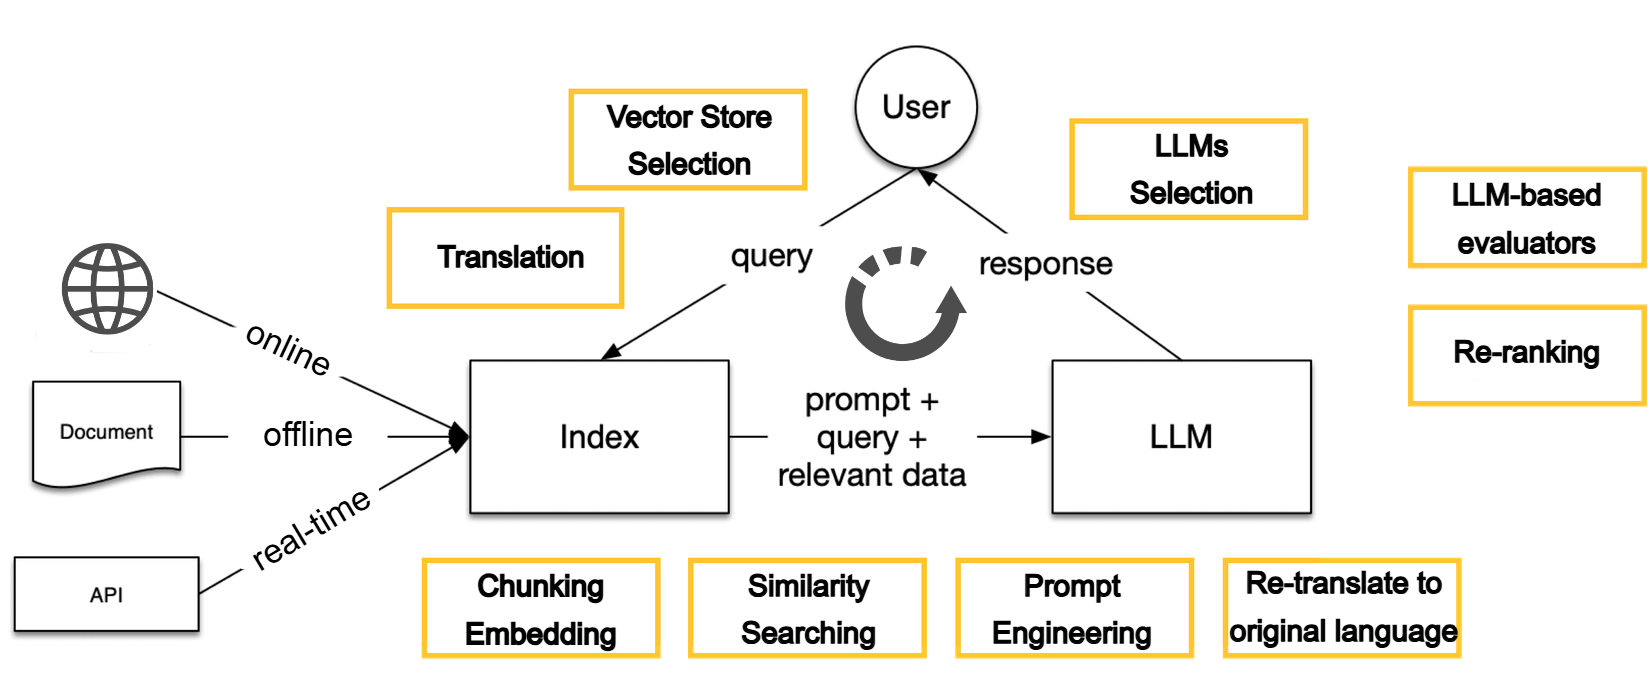
\includegraphics[width=\linewidth]{./figures/rag_components.png}
    \caption{The composition of the system's RAG pipeline}
\end{figure}
This figure demonstrates the overall processes that are executed in the system, incorporating the following concepts:
\begin{itemize}
    \item Vector Store (Index): Is a type of a database suitable for storing large volumes of documents that needs to be queried efficiently. This repository represents the Entreprise Knowledge Base.
    \item Data ingestion: Refers to the sources from which the knowledge base can be augmented.
    \item Embeddings Model: is an algorithm that transforms text (or other data) into numerical representations called embeddings, capturing semantic and syntactic information, which enables the vector store to find the most relevant information based on a query.
    \item Generative AI model (LLM): This is a type of a ML model that can analyze textual input and generate output accordingly.
    \item Prompt: A set of instructions and other information that elicits a certain output or behavior from the generative model.
    \item Other AI models: Used for translating text between languages, and re-ranking and compressing the retrieved context.
\end{itemize}
The following subsections are dedicated to the exploration of these elements and selecting concrete tools from these concepts.
\subsection{Vector Stores}
'Vector Store' refers to a type of database responsible for the storage and indexation of documents and other unstructured data in a numerical representation suitable for retrieving relevant parts from large volumes of data through similarity searching algorithms.
\begin{quote}
    "Traditional databases are made up of structured tables containing symbolic information. For example, an image collection would be represented as a table with one row per indexed photo. Each row contains information such as an image identifier and descriptive text. Rows can be linked to entries from other tables as well, such as an image with people in it being linked to a table of names.

    AI tools, like text embedding (word2vec) or convolutional neural network (CNN) descriptors trained with deep learning, generate high-dimensional vectors. These representations are much more powerful and flexible than a fixed symbolic representation, as we’ll explain in this post. Yet traditional databases that can be queried with SQL are not adapted to these new representations. First, the huge inflow of new multimedia items creates billions of vectors. Second, and more importantly, finding similar entries means finding similar high-dimensional vectors, which is inefficient if not impossible with standard query languages."  \cite{faissess}
\end{quote}
This specific type of database provides many functionalities and processes pertinent to the functioning of a RAG pipeline, which are explored in the following subsections.
\subsection{Chunking}
First of all, when indexing large documents into the knowledge base, one should consider the size of this contiguous information and the context window limitation of LLMs, as each model has some limit on the amount of information it can receive as context. In these conditions, a chunking of documents should be implemented before the embedding and storing phases. This technique allows to divide documents into smaller passages, while marking these with metadata (document id, order etc...) which would allow the vector store to structure and store these chunks as if they were a monolithic record.\newline
The following figure demonstrates the initial steps when a new data source is being recorded into the knowledge base.
\begin{figure}[H]
    \centering
    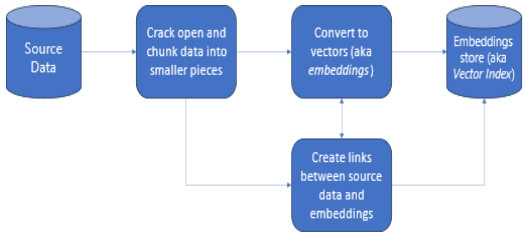
\includegraphics[width=.7\linewidth]{./figures/chunking-embedding-diagram.png}
    \caption{Embedding Document Chunks Diagram. (Microsoft, 2023)}
    \begin{flushleft}
        When loading new information into the vector store, a segmentation of the content needs to occur before transforming it into numerical representation. The chunking phase achieves this by splitting the document into a fixed length chunks, creating links between them and then passes to next phase of vectorization or embeddings generation, which is discusses below.
    \end{flushleft}
\end{figure}
\subsection{Vectorization}
Embedding vectors, as in vector store, are arrays of floating-point numbers produced by embeddings models. The output of these models captures the semantics of the vectorized text. This representation is suitable for RAG applications because these embeddings are computed in a way that semantically similar information have similar values, which allows for efficient indexation and similarity search algorithms' implementation.
\begin{figure}[H]
    \centering
    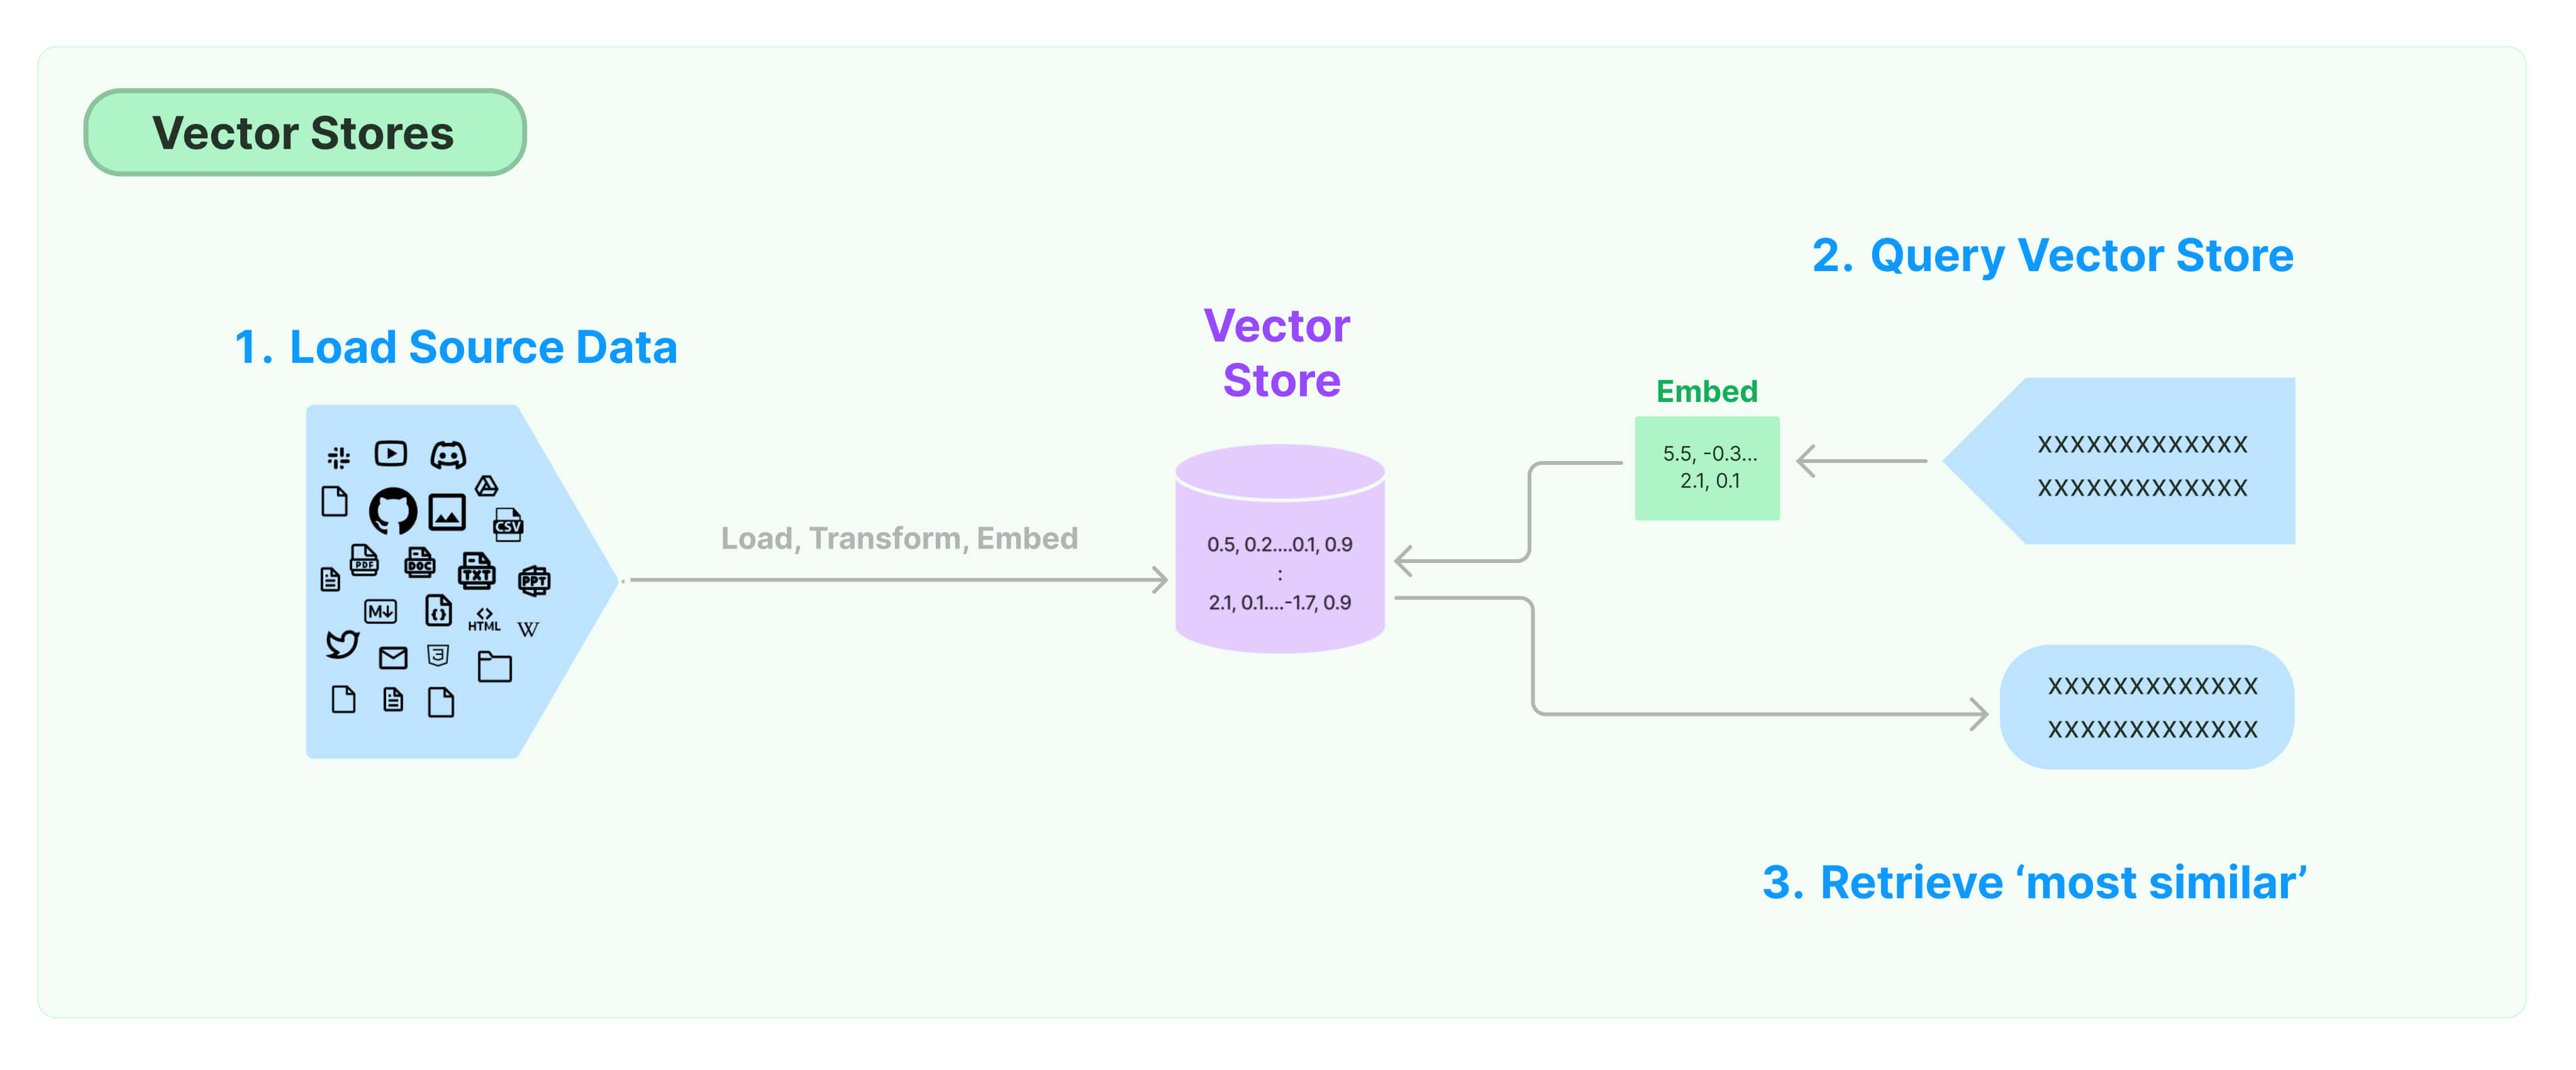
\includegraphics[width=\linewidth]{./figures/vectorstore.jpg}
    \caption{Vector Store Process Diagram \cite{langchainvectorstore}}
    \begin{flushleft}
        \small This figure illustrates the functioning of an embedding model in a vector store environment, transforming source data to numerical representations, and embedding queries to retrieve the most similar vectors.
    \end{flushleft}
\end{figure}
\subsection{Indexation}
The term indexation refers to the organization and storage of the generated embeddings to optimize the retrieval process afterwards. There are many indexation methods, such as Flat, Hierarchical, Quantized methods, etc... The exploration of these different methods is beyond the objectives of this internship, but these different indexation strategies share a common aim of storing chunks in a data structure, in a way that the similarity search algorithms (discussed below) can retrieve the relevant context efficiently and accurately.
\begin{figure}[H]
    \centering
    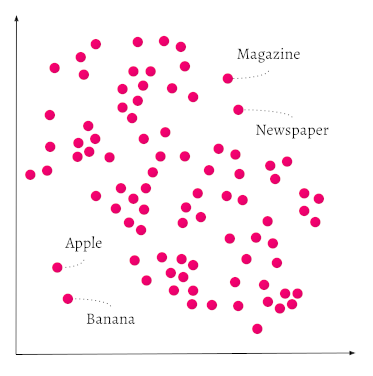
\includegraphics[width=.5\linewidth]{./figures/vs-indexation.png}
    \caption{Vector Store Index Visualization \cite{weaviateindexing}}
    \begin{flushleft}
        \small This figure demonstrates how some word embeddings are indexed so that semantically similar elements are grouped together.
    \end{flushleft}
\end{figure}
\subsection{Similarity Search}
In addition to the ability to index and store documents' sections in a suitable format, the vector store index should also be able to search these elements (and then decode them back into their original textual form). This is achieved through similarity search algorithms often implemented as constituent functionalities with the vector store. These functions return a number of passages semantically similar to the search term and is achieved due to the concept of distance calculation between vectors in data analysis.\newline
The following figure represents the different metrics of these algorithms.
\begin{figure}[H]
    \centering
    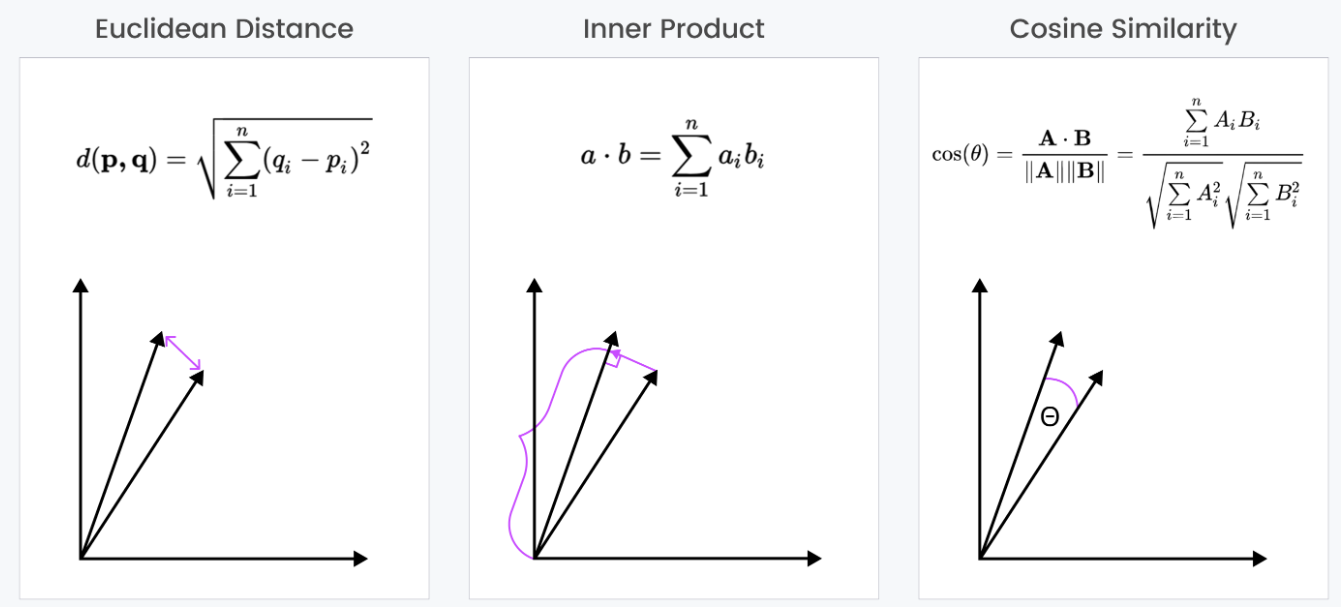
\includegraphics[width=\linewidth]{./figures/vector-distance-metrics.png}
    \caption{Similarity Metrics for Vector Search \cite{zsimilaritymetrics}}
\end{figure}
The Euclidean Distance metric is more suitable when looking for precise differences in numerical values, achieving results similar to exact word matching, which is irrelevant in the context of RAG. The Inner Product metric is more advanced in a way that it focuses on calculating the difference between the vectors' directions more than their magnitudes, but still it prioritizes results with similar lengths to the input query. The cosine similarity metric, which is the most suitable algorithm for our case, only calculates similarity based on the direction of vectors rather than their magnitude, which means that the embeddings which will be retrieved from the knowledge base will be the ones with the most semantic similarity, rather than length similarity, to the user-provided query embeddings.
\subsection{Retrieval Re-ranking}
Considering the context window limitation mentioned in the chunking subsection, and the complex task of retrieving the most relevant context, it is worth employing an additional step to the similarity search metrics mentioned in the previous subsection. This is because cosine similarity, even though an efficient metric for retrieving the context, still has limitations when dealing with complex natural language content.
\begin{figure}[H]
    \centering
    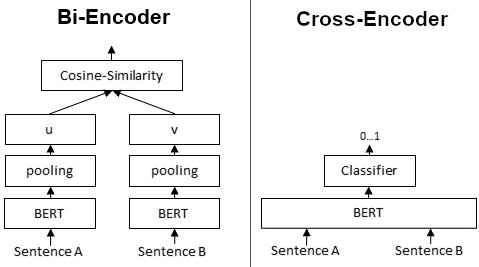
\includegraphics[width=.8\linewidth]{./figures/Bi_vs_Cross-Encoder.png}
    \caption{Bi-encoder VS Cross-encoder \cite{bivscrossencoders}}
\end{figure}
The post-retrieval process being discussed allows to compress the retrieved information from the basic similarity search algorithm by employing a neural network to further re-rank and drop irrelevant or recurrent parts from the retrieved information. This type of neural network, called Cross-Encoder Re-ranking, captures the order and relationships between the words in the query and the given chunk simultaneously, and predicts its relevance to the question.
\subsection{Large Language Models}
Text Generative AI encompasses models capable of artificially producing textual content based on a prompt (discussed in the following subsection). It can allude to the tasks of next word suggestions, summarization, rewriting in different tones, cross-language translation, question answering, text or code generation etc...
Large Language Models (LLMs) constitute a subset of AI models that leverage massive natural language training datasets. Prominent examples of such models include GPT-3, Gemini, and Llama-3. While some of these models have been extended to incorporate multimodal capabilities (multimedia content), their core functionality remains rooted in language processing and generation, providing a robust foundation for the required tasks in a RAG pipeline.
\begin{figure}[H]
    \centering
    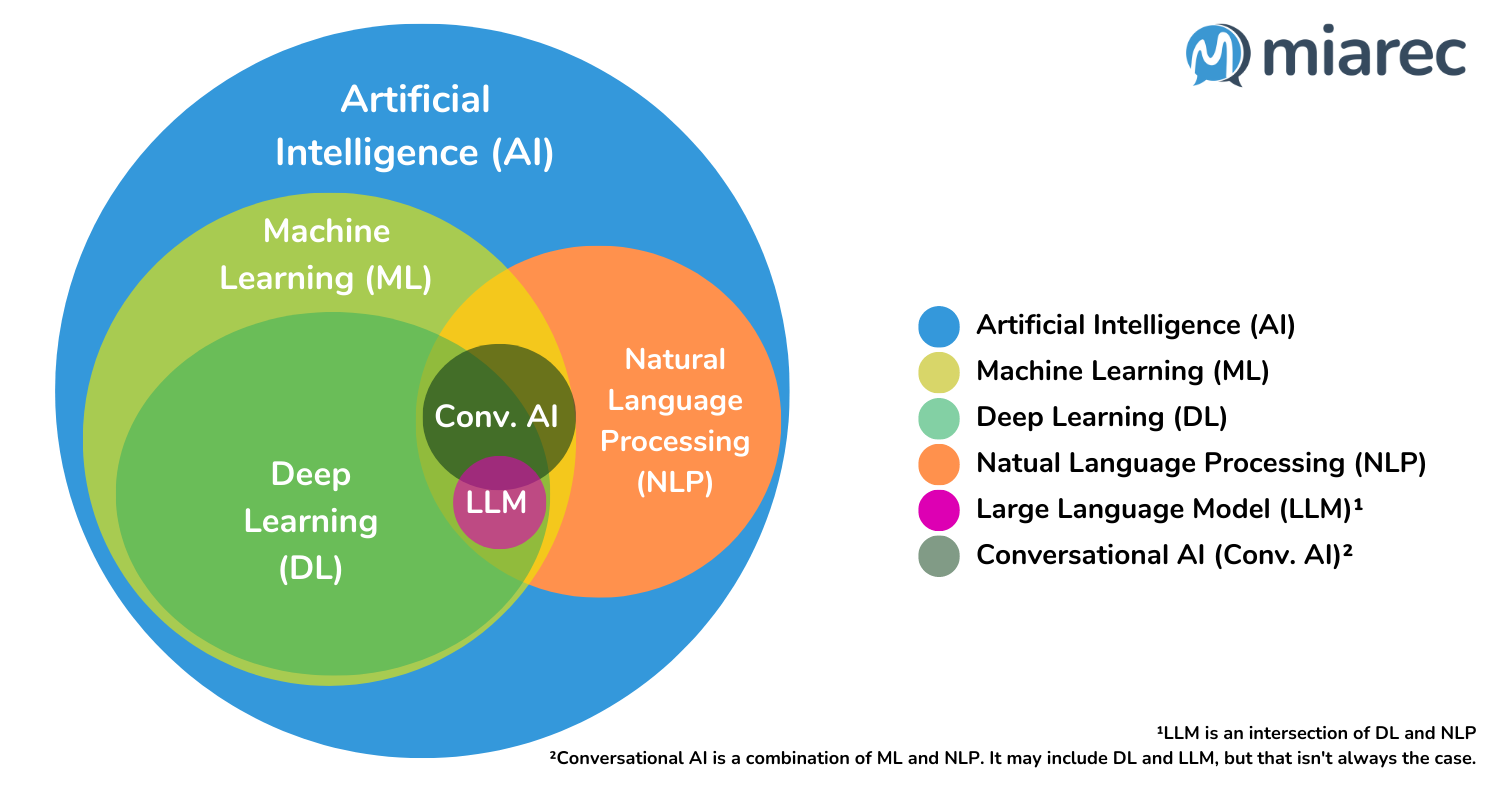
\includegraphics[width=.97\linewidth]{./figures/genai-relation-diagram.png}
    \caption{Relationship between AI, ML, DL, NLP, and Conversational AI terms \cite{aidomainsrel}}
    \begin{flushleft}
        \small This figure illustrates the relationship between AI domains. In this project, our focus is more onto LLMs (we use the term "LLM" interchangeably to mean "Large Language Model" that may or may not be "Conversational AI"), which are ML models able to hold chat history when answering consecutive queries.
    \end{flushleft}
\end{figure}
LLMs represent the principal component of a RAG system. It acts as tool that understands user prompts' context and generate textual responses accordingly. Essentially, these models are transformer-based, which allows them to learn complex relationships between words in sentences thanks to their attention mechanisms.
\begin{figure}[H]
    \centering
    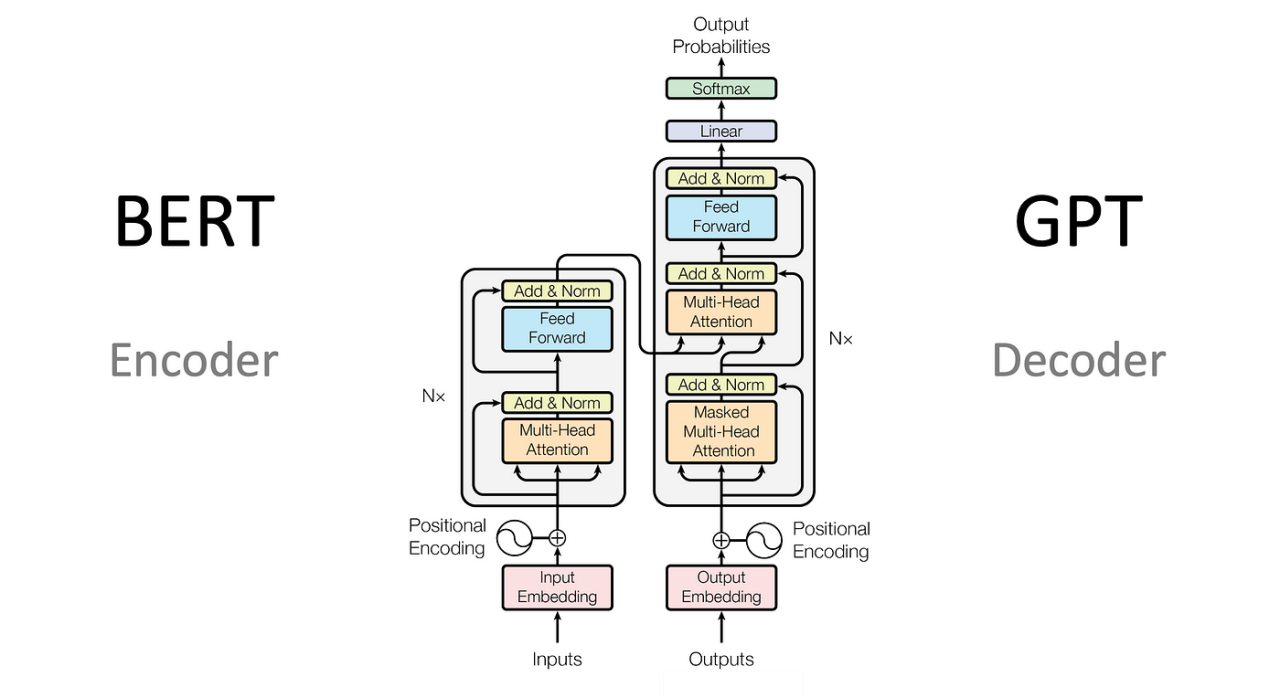
\includegraphics[width=\linewidth]{./figures/The-Transformer-model-architecture.png}
    \caption{An illustration of main components of the transformer model from the original paper \cite{transformersarch}}
\end{figure}
To provide some cursory understanding of the functioning of these models, the following are the main steps that such architecture involves:
\begin{itemize}
    \item \textbf{Input Embedding:} The transformer first converts the input text into a series of numerical representations,  which are then passed through a positional encoding layer. This layer adds information about the word’s position in the sentence, which is important because word order matters in a language like English.
    \item \textbf{Encoder Layers:} The core building block of the transformer encoder is the “encoder layer”.  An encoder layer typically consists of two sub-layers: a multi-head attention layer and a feed-forward layer.
    \item \textbf{Multi-Head Attention Layer:} The multi-head attention layer allows the model to attend to different parts of the input sentence simultaneously. This is important for understanding the relationships between words in a sentence.
    \item \textbf{Feed Forward Layer:} The feed-forward layer is a simple neural network that further processes the information from the attention layer.
    \item \textbf{Decoder Layers:} After the encoder has processed the input text, the decoder generates the output text. The decoder also uses encoder layers, but with an additional masked multi-head attention layer. This layer prevents the decoder from attending to future words in the output sentence, which would allow it to “cheat” by looking ahead.
    \item \textbf{Softmax Layer:} The softmax layer converts the decoder's output into a probability distribution over all the words in its vocabulary. This allows the model to predict the next word in the sentence for instance.
\end{itemize}
We can make use of these LLMs' capabilities and the retrieval phase discussed in the previous subsections, which when combined, serve to leverage the retrieved information to generate more insightful responses.
\subsection{Prompts and Prompt Engineering}
Prompt Engineering (PE) techniques play a crucial rule in the context of RAG and LLMs in general, by acting as a link between the retrieval and the generation phases. It refers to how the model is prompted, i.e. what does it receive as input. It may include several instructions to the LLM that guides it on how to perform the generation stage. It also can include different parts or steps, such as passing the retrieved context or chat history directly into the prompt, provide it with examples which it should consider when providing answers, or instruct it on how long the answer should be or in which tone it should respond.
\begin{figure}[H]
    \centering
    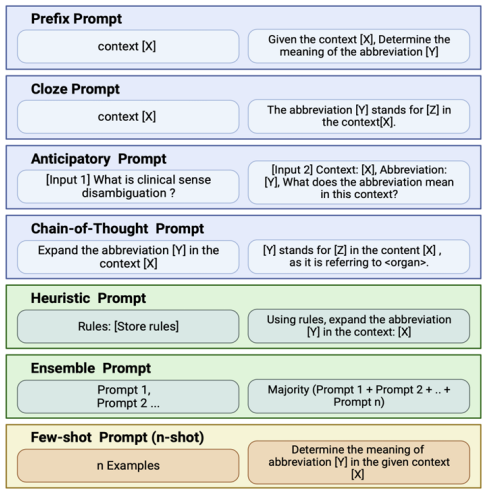
\includegraphics[width=\linewidth]{./figures/prompt-types.png}
    \caption{Types of Prompts: [X]: context, [Y]: Abbreviation, [Z]: Expanded Form
    \cite{prompts}}
    \begin{flushleft}
        The figure above provides many types and examples of prompts. We can distinguish two characteristics: instructions and placeholders.\newline
        Instructions, such as "Given the context [], Determine the meaning of []" and "Determine the meaning of [] in the given context []", allow to control how the AI model processes its input when generating answers, and help instruct the model to limit its knowledge based on the retrieved context for our case.\newline
        The placeholders, "[X]" and "[Y]" for example, allow to interpolate textual information that changes each time a model is called. These placeholders allow to insert user queries alongside our chosen instructions, and pass context relevant to the query each time, in format intelligible to the LLMs.
    \end{flushleft}
\end{figure}
\subsection{Generation Re-ranking}
This final post-generation phase process aims to prioritize better answers by calculating specific scores for each model's response generation. There are mainly three metrics for this type phase.
\subsubsection{Faithfulness}
This metric allows to measure the hallucination of a model and de-prioritizes its answer. It achieves this by calculating the proportion of the claims which can be inferred from the retrieved context against the total number of claims, which can be either from the context or not (hallucination).
\subsubsection{Answer Relevancy}
Similarly to the Faithfulness metric, which focuses on the generated answer its relation with the retrieved context, this metric assesses the pertinence of the generation phase's outcome to the initial prompt. This metric is calculated by reverse engineering the RAG pipeline: Given a generated answer, LLMs attempt to speculate some variants of questions that can be asked to obtain that generation, and then calculates the mean cosine similarity between those speculated questions and the actual question.
\subsubsection{Model Feedback}
This metric allows to capture the users' feedback and measure the trust our users have in AI models. It measures this by allowing each user to rate an answer in a scale from 1 to 5. These accumulated scores are then divided by the number of feedbacks given to a single LLM. In addition to this, a model which has no feedback is given a score of 3 to make it neither prioritized nor de-prioritized  over other models.

\section{Conclusion}
This chapter has identified the key components that will make up our system, highlighting the interaction between them. In summary, to implement a functional RAG pipeline, one needs to orchestrate a Vector Store with methods for knowledge augmentation, similarity search methods to retrieve relevant information, LLMs to generate responses, and prompt engineering to control LLMs' behavior.\newline
Having a clear understanding of these individual parts is essential, as the following chapter discusses the implementation phase in detail.

\chapter{Implementation}

\section{Introduction}
This chapter details the implementation process of the solution discussed in the previous chapter: The work environment, tools and libraries employed to accomplish the tasks, and the technical aspects of design choices execution.

\section{Workstation}
This section identifies the characteristics, both hardware and software, of the computer system on which this project was implemented.
\bigskip
\subsection{Hardware}
\smallskip
\begin{itemize}
    \item Device : DELL Inspiron 3593
    \item Processor : Intel(R) Core(TM) i7-1065G7 CPU @ 1.30GHz   1.50 GHz
    \item RAM : 24 GB
    \item GPU : NVIDIA GeForce MX230
\end{itemize}
\medskip
\subsection{OS and Software}
\smallskip
\begin{itemize}
    \item OS : Debian trixie inside a Windows Subsystem for Linux (WSL2) VM
    \item Source-code Editor : Visual Studio Code (with extensions to enable interacting with WSL, Jupyter Notebooks and Python virtual environments) + NeoVim
    \item Web Browser : Microsoft Edge (for web application testing and troubleshooting)
    \item Drivers and Toolkits : NVIDIA GPU driver + CUDA Toolkit among others
\end{itemize}

\section{Components}
In this section, we research available tools making it possible to develop the different functionalities, provide comparison between alternatives when choices were made, go through how they were implemented and end up with testing the effectiveness of the developed solution in addition to laying out its unfortunate limitations.
\subsection{Libraries and Frameworks}
\subsubsection*{Web Interface and Services}
There is a plethora of frameworks of this kind, from customary JavaScript frameworks (React, Angular, Vue) to others designed to enable faster delivery of interactive web apps (such as Streamlit and Chainlit).\newline
The choice was made to use Streamlit as it provides a much faster way to develop LLM chat interfaces than JS frameworks, while also being more advanced than Chainlit in terms of flexibility and building custom interfaces by supplying developers with many customizable and ready-to-use interface components like chat and message containers.
\begin{figure}[H]
    \centering
    
\includegraphics[width=.5\linewidth]{./figures/streamlit-logo.png}
    \caption{Streamlit logo.}
\end{figure}
We can look through its app gallery to find an abundance of templates that provide many examples of built apps which interact with LLMs, LangChain and other frameworks.
\begin{figure}[H]
    \centering
    
\includegraphics[width=\linewidth]{./figures/streamlit-app-gallery.png}
    \caption{Streamlit App Gallery.}
\end{figure}
\subsubsection*{RAG Pipeline Development}
There are a few frameworks enabling developers to interact with LLMs and RAG pipelines, each of which provide different integrations with external APIs and tools: LangChain, LlamaIndex, Haystack, Langroid.\newline
The choice was made by 3S project coordinators to use LangChain for their solution. It is a great choice given that this platform provides all the tools to build complex RAG pipelines and personalize the different steps of these pipelines. Also, since its emergence in October 2022, this library has gained remarkable prominence with courses available on DeepLearning.ai, tutorials from NVIDIA, OpenAI, Google and others in addition to the exhaustive documentation available online.
\begin{figure}[H]
    \centering
    
\includegraphics[width=.5\linewidth]{./figures/langchain-logo.png}
    \caption{LangChain logo}
\end{figure}
This framework has all the required components to build the most advanced RAG pipelines: Data loading from various sources, LLM and vector store integrations from different providers (both locally and on the cloud), prompt templates for different LLMs and tasks, etc...
\begin{figure}[H]
    \centering
    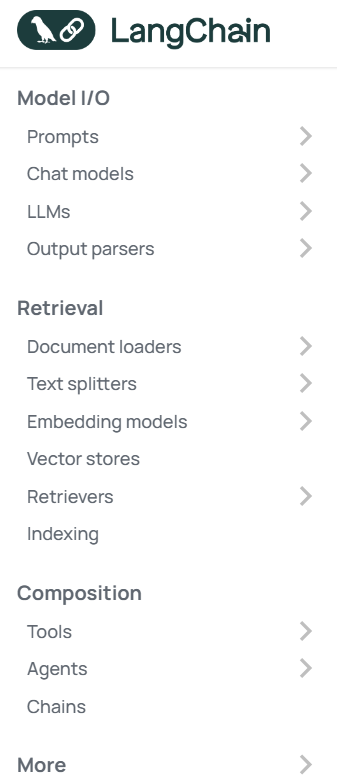
\includegraphics[width=.45\linewidth]{./figures/langchain-components.png}
    \caption{LangChain Components. (\href{https://python.langchain.com/v0.1/docs/modules/}{LangChain Documentation})}
\end{figure}
\subsection{Large Language Models}
There is a plethora of models of this type, both closed and open source, with many ways to access and use them.
\subsubsection{Local}
Many open-source LLM variants are available on Hugging Face Models Hub, as it is the main developer of the 'transformers' Python library.
\begin{figure}[H]
    \centering
    
\includegraphics[width=0.4\linewidth]{./figures/hf-logo.png}
    \caption{Hugging Face logo. \href{https://huggingface.co/models}{[Hugging Face models Hub]}}
\end{figure}
\begin{quote}
    "The Hugging Face Hub hosts many models for a \href{https://huggingface.co/tasks}{variety of machine learning tasks}. Models are stored in repositories, so they benefit from \href{https://huggingface.co/docs/hub/repositories}{all the features} possessed by every repo on the Hugging Face Hub. Additionally, model repos have attributes that make exploring and using models as easy as possible."  (\href{https://huggingface.co/docs/hub/models}{[Hugging Face Models Hub documentation]}, 2024)
\end{quote}
We can find an abundance of pre-trained LLMs downloadable from the HF Hub.
\begin{figure}[H]
    \centering
    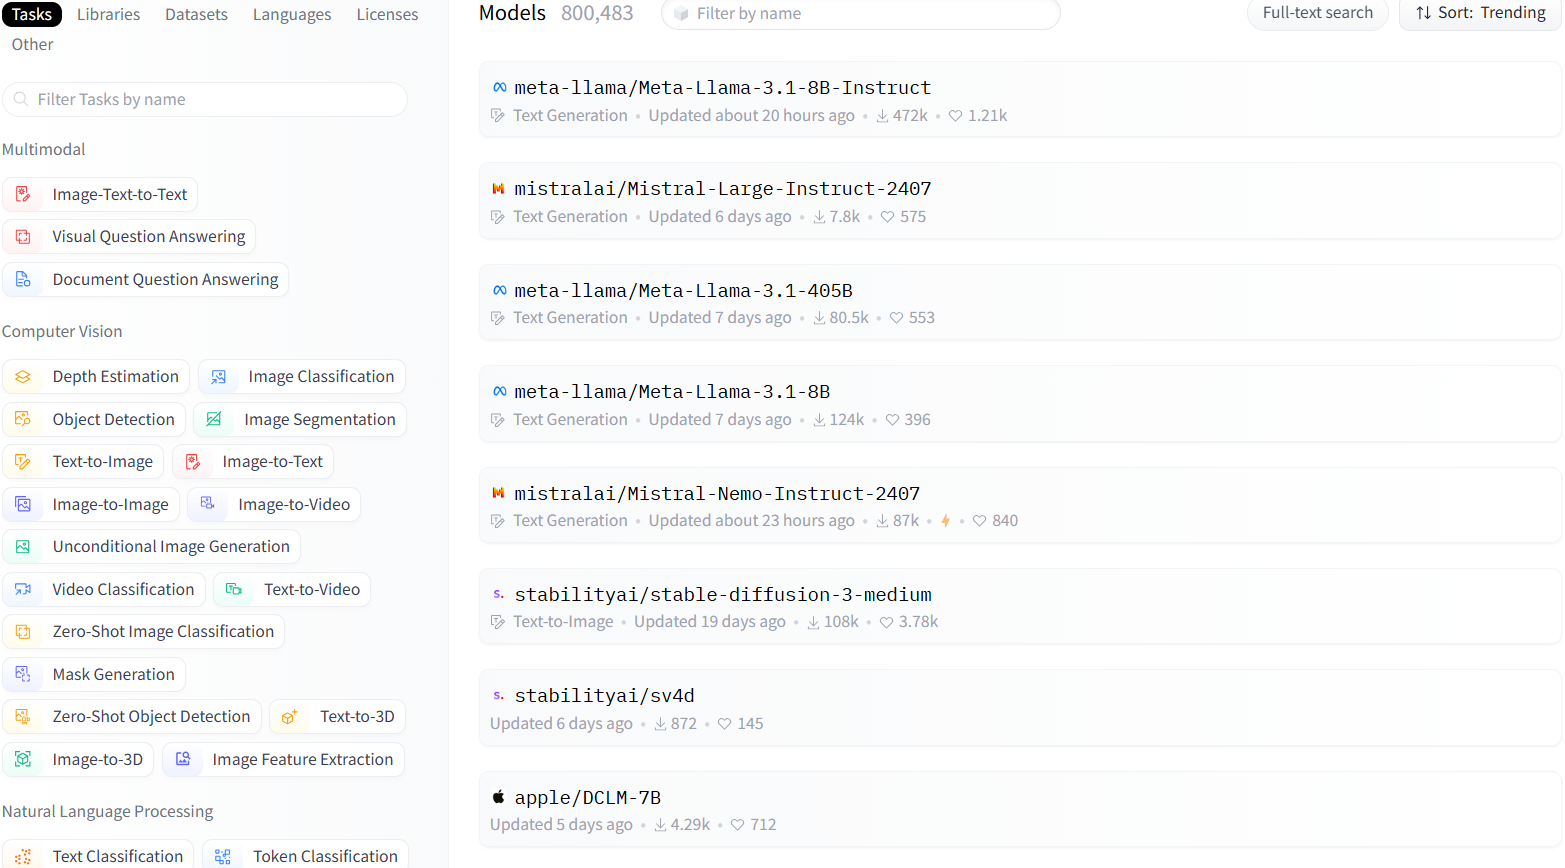
\includegraphics[width=.85\linewidth]{./figures/hf-models.png}
    \caption{HF Hub models, categorized by their tasks. \href{https://huggingface.co/models}{[Models - Hugging Face]}}
\end{figure}
This method allows the free utilization of a pre-trained model without being confined to cloud-platforms and their plans.
\subsubsection{Cloud-based Solutions}
In addition to the previous method, many companies behind Large Language Models development provide APIs or cloud-based environments to access their models. Some of the most popular options include OpenAI API, Google Cloud Vertex AI, Anthropic, Cohere, FireworksAI, MistralAI, TogetherAI, GroqCloud among others.\newline
This method, in contrast to running models locally, does not come with the pre-requisites of expensive hardware or delayed answer generation. Even though these solutions are paid services, most provide free trials and some of the available free plans only has a limit on daily and monthly usage, and is usually enough for personal usage. In addition to this, some of these cloud environments provide many models to use. For instance, FireworksAI allows to use Llama-3, Yi-Large, Mixtral, while TogetherAI provides models such as Qwen-2, Gemma (open-source version of Google's model, Gemini), Phi-2, Nous Capybara, and many others, all from within a single platform.
\begin{figure}[H]
    \centering
    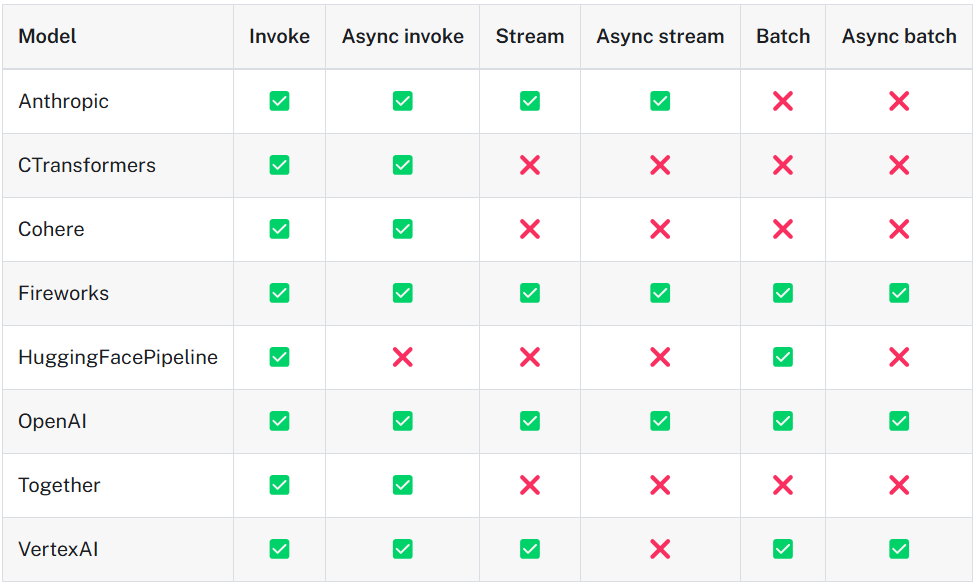
\includegraphics[width=\linewidth]{./figures/langchain-llm-integrations.png}
    \caption{LangChain Integrations with LLMs cloud providers. \href{https://python.langchain.com/v0.1/docs/integrations/llms/}{[Langchain Documentation - LLMs]}}
    \begin{flushleft}
        \small The previous list presents a subset of the integrations provided by Langchain. In addition to the aforementioned items, MistralAI and GrokCloud were integrated in the system to provide a plethora of Large Language Models suitable for Retrieval-augmented Generation. This solution also allows for some customization options through their web interfaces and API function parameters, even though limited when compared to local implementation.
    \end{flushleft}
\end{figure}
\begin{figure}[H]
    \centering
    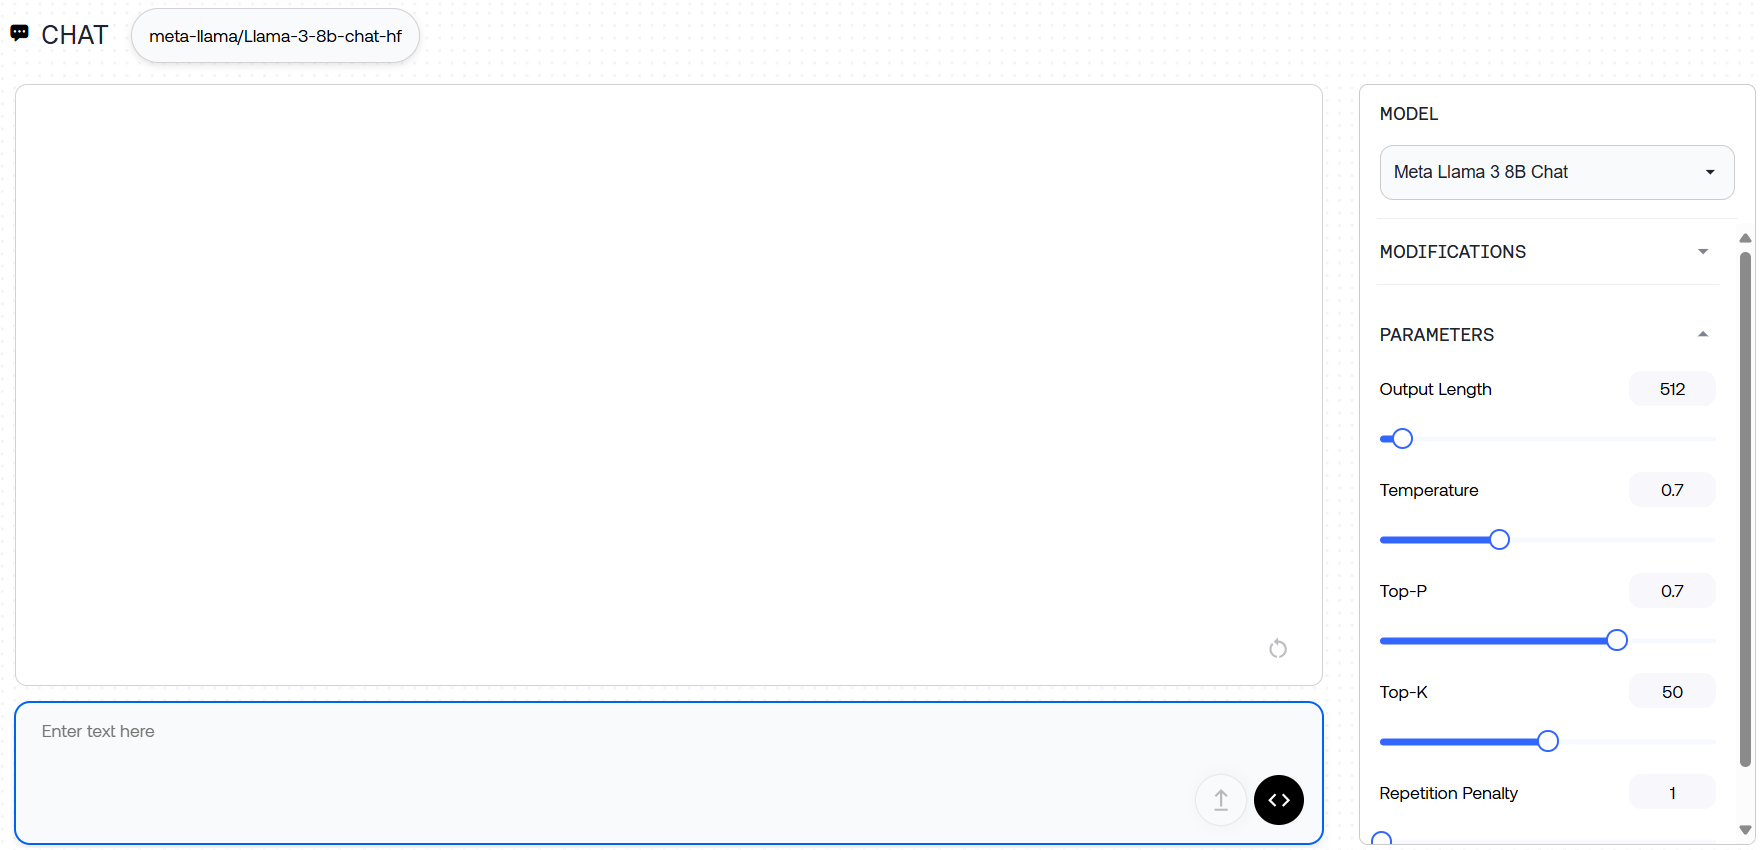
\includegraphics[width=\linewidth]{./figures/togetherai-playground.png}
    \caption{TogetherAI playground web interface. \href{https://api.together.ai/playground}{TogetherAI Playground service}}
    \begin{flushleft}
        This figure demonstrates an example of a cloud-based environment providing multiple LLM's customization options and parameters, allowing to customize and use a Llama model without locally downloading it.
    \end{flushleft}
\end{figure}
\subsection{Vector Stores}
There are many vector stores and embedding models to choose from, which we will look through their differences in this subsection.\newline
The choice of the most suitable vector store solution was based on four criteria mainly:
\begin{itemize}
    \item Self-hosting: This means that the vector store will be managed locally on the same computing infrastructure as the web server. This is opposed to a cloud-based deployment, which comes with the drawbacks of higher latency, possible network errors and high-costs.
    \item Latency: This refers to the performance and speed of similarity searching algorithms which are provided by the vector store and its ability to index and handle large volumes of data with the utilization of GPU parallel computing features.
    \item Accuracy: The relevance of retrieved data to the actual searched query. Often, this has a reverse relation with latency, as more accurate results take longer to be achieved.
    \item Documentation: Online Documentation and community forums that can guide on how to use the database efficiently.
\end{itemize}
\begin{table}[H]
    \begin{tabular}{|c|c|c|c|c|}
        \hline
        \textbf{\textcolor{darkgray}{Vector Store}} & \textbf{\textcolor{darkgray}{Self-hosting}}               & \textbf{\textcolor{darkgray}{Latency}} & \textbf{\textcolor{darkgray}{Accuracy}} & \textbf{\textcolor{darkgray}{Documentation}} \\  \hline
        \textbf{FAISS}                              & \textcolor{green}{\ding{52}}                              & \textcolor{green}{\ding{52}}           & \textcolor{green}{\ding{52}}            & \textcolor{red}{\ding{56}}                   \\ \hline
        \textbf{Pinceone}                           & \textcolor{red}{\ding{56}}                                & \textcolor{green}{\ding{52}}           & \textcolor{red}{\ding{56}}              & \textcolor{green}{\ding{52}}                 \\ \hline
        \textbf{Chroma}                             & \textcolor{green}{\ding{52}} / \textcolor{red}{\ding{56}} & \textcolor{green}{\ding{52}}           & \textcolor{red}{\ding{56}}              & \textcolor{green}{\ding{52}}                 \\ \hline
        \textbf{Lance}                              & \textcolor{green}{\ding{52}}                              & \textcolor{red}{\ding{56}}             & \textcolor{red}{\ding{56}}              & \textcolor{red}{\ding{56}}                   \\ \hline
    \end{tabular}
    \caption{Comparison of popular vector databases}
\end{table}
After careful consideration, FAISS vector store was selected due to its high performance and accuracy in comparison to alternatives. It leverages the GPU-enabled CUDA toolkit, and provides a state-of-the-art implementation of similarity searching algorithms based on this structure.
\begin{figure}[H]
    \centering
    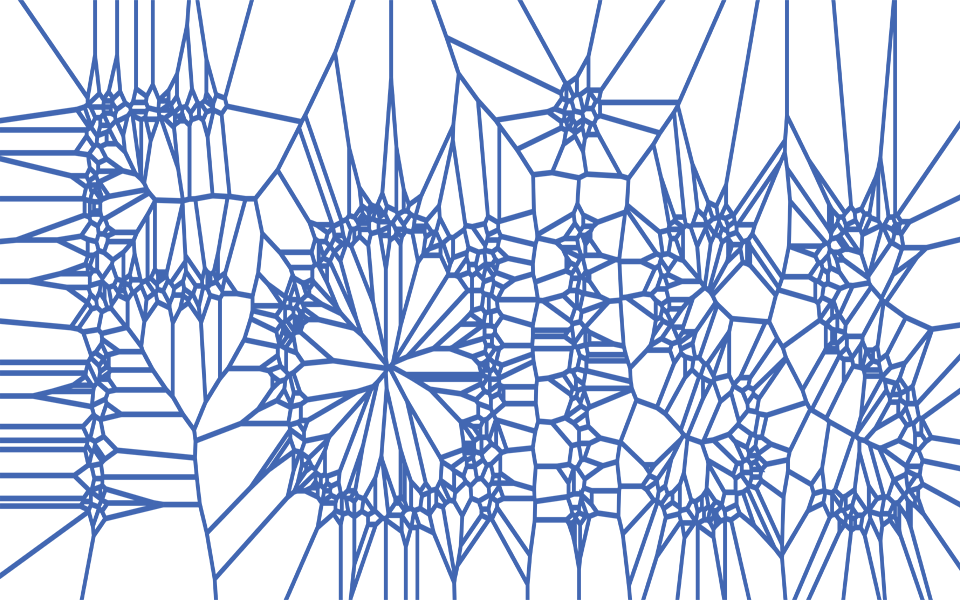
\includegraphics[width=.5\linewidth]{./figures/faiss_logo.png}
    \caption{FAISS logo.}
\end{figure}
\begin{quote}
    Facebook AI Similarity Search (FAISS) is an open-source library providing the basic data structures suitable for storing the vector store both in memory or on disk, with implementations of nearest neighbor search and k-selection algorithms designed specifically to efficiently handle large data sets, 8.5x faster than previous methods.
\end{quote}
\subsection{Embedding Model}
We have highlighted in the previous chapter the importance of an embedding algorithm that minimizes the loss of semantics when converting textual data to embedding vectors. In addition to this, considering that a vector store once initialized with an embedding model, can no longer replace it with another without its contents being wiped out completely. For this purpose, it would be a bad choice to consider cloud solutions, as these models may be unavailable in some cases (network or provider failure, expiration of tokens...).\newline
The best choice in this case, as in vector store's choice, is to select a suitable model which is available offline (as in self-hosting). This will avoid foreseeable failures and limit problems.\newline
This redirects us to the Hugging Face Hub where we can find many embedding models, which are available through the sentence transformers repository.
\begin{figure}[H]
    \centering
    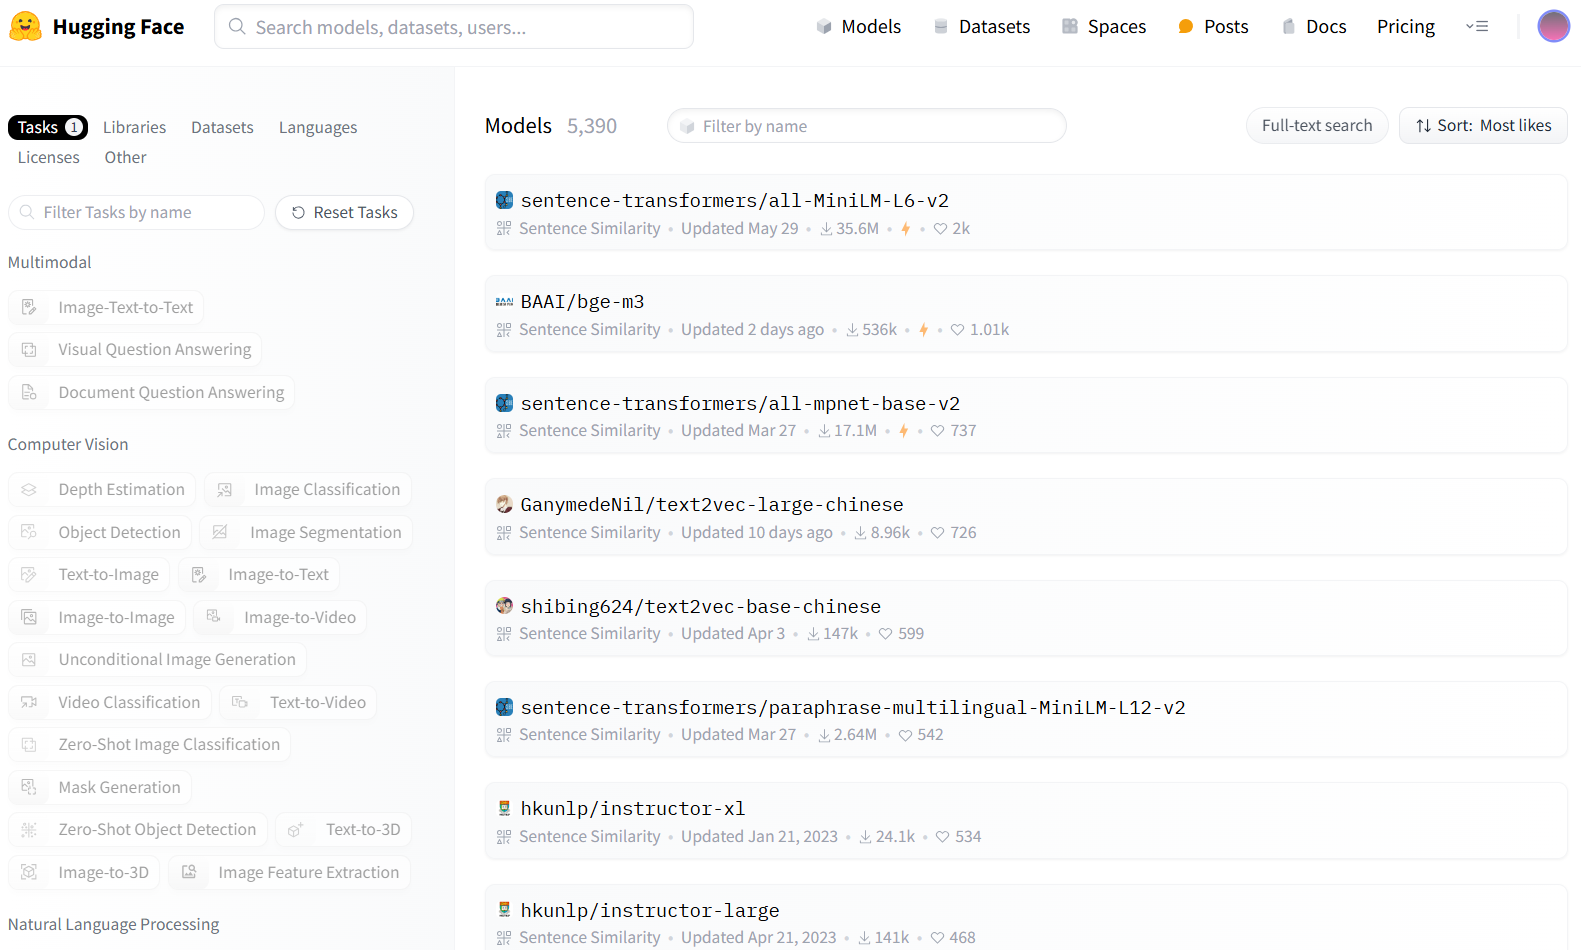
\includegraphics[width=.85\linewidth]{./figures/hf-embedding-models.png}
    \caption{A list of Embedding models from HF Hub. \href{https://huggingface.co/models?pipeline_tag=sentence-similarity&sort=likes}{Models | Hugging Face}}
\end{figure}
This list contains two of the most popular choices, which are "all-MiniLM-L12-v2" and "all-mpnet-base-v2", the first of which makes a better choice when working in a limited environment while not paying much attention to retaining semantics (faster embedding generation and smaller size), while the second one, "all-mpnet-base-v2", is the more suitable choice for our case due to, even with its larger footprint, its capability to capture most of the semantics and meanings of sentences.
\begin{figure}[H]
    \centering
    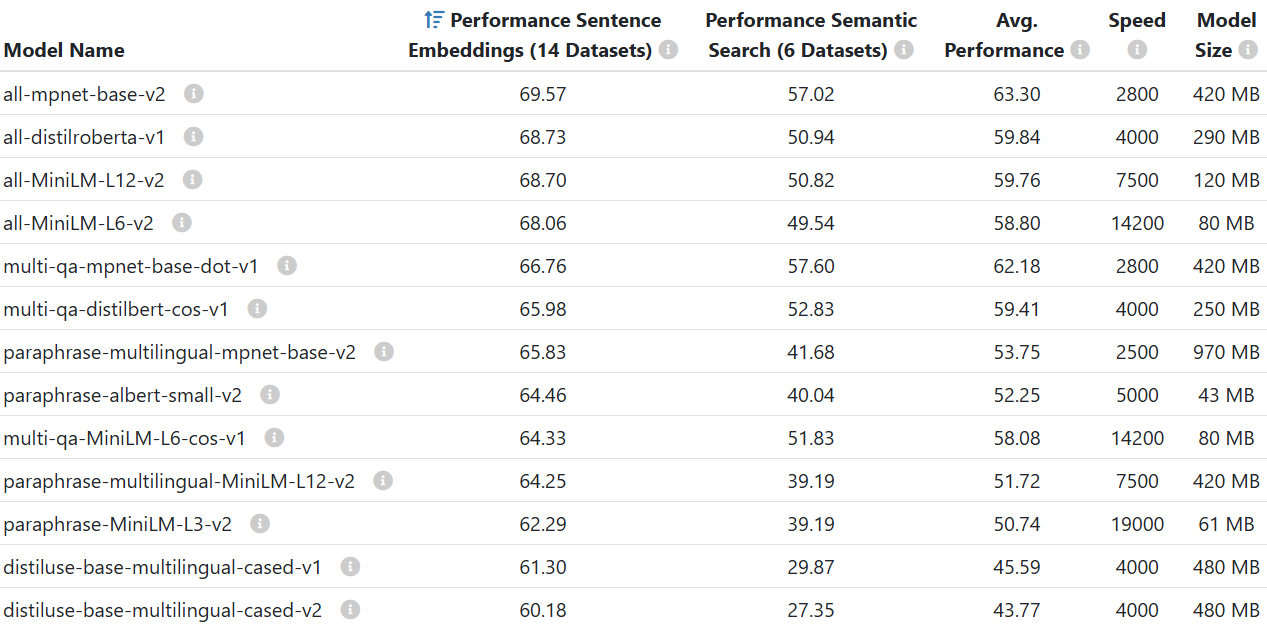
\includegraphics[width=\linewidth]{./figures/embedding-modes-performance.png}
    \caption{Sentence-Tansformers model performance comparison \href{https://sbert.net/docs/sentence_transformer/pretrained_models.html}{[Pre-Trained Sentence Transformers models' performance]}}
    \begin{flushleft}
        This table provides an overview of an extensive evaluation for the quality of a number of embeddings models. These models are ranked based on many metrics: performance of encoding generation over diverse domains, semantic search, speed and size.
    \end{flushleft}
\end{figure}
\begin{quote}
    "The all-* models were trained on all available training data (more than 1 billion training pairs) and are designed as general purpose models. The all-mpnet-base-v2 model provides the best quality, while all-MiniLM-L6-v2 is 5 times faster and still offers good quality."  (\href{https://sbert.net/docs/sentence_transformer/pretrained_models.html}{[Sentence Transformers documentation]})
\end{quote}

\section{Incorporating into a RAG System}
After introducing the frameworks and tools which would allow us to build a RAG system, it is necessary to discuss the implementation details of these elements and how they were incorporated together.\newline
This section is dedicated to showcasing how these components interact together in the implemented solution.

\subsection{Data Ingestion Methods}
The first essential part of the project is to allow the on-demand ingestion of data and new information into the vector store.\newline
For this purpose, various file formats and online web scraping and fetching methods have been implemented; LangChain, as seen in the previous section, provides a "Document loaders" section in its "Retrieval" toolbox. These tools provide many tutorials and helpful functions to implement document loading and chunking from various sources, which has allowed to accomplish the required methods to satisfy the coordinating teams at 3S.
\begin{figure}[H]
    \centering
    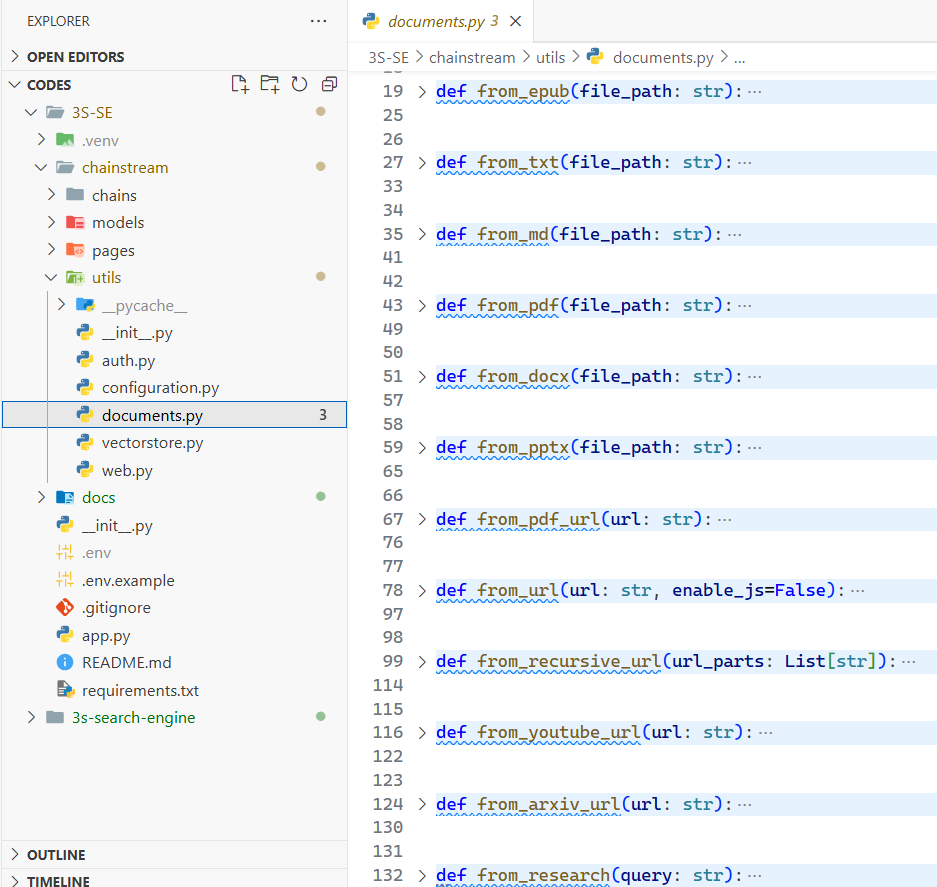
\includegraphics[width=\linewidth]{./figures/data-ingestion-methods.png}
    \caption{Various data ingestion methods}
\end{figure}
To make it more comprehensible, here is a short description of what each of these methods do:
\begin{itemize}
    \item Web Pages (from\_url, from\_recursive\_url): Allowing to read a single page from a given URL, or a page and its child pages recursively, supporting static and dynamic web content.
    \item Arxiv Research Papers (from\_arxiv\_url): Allows to read content directly from an arxiv URL, conserving metadata like author, dates, etc...
    \item Youtube Content (from\_youtube\_url): Transcribes a video uploaded on YouTube and constructs a document from a given URL.
    \item Generative Research (from\_research): Utilizes \href{https://gptr.dev/}{GPT Researcher}, a tool that allows to, given a question, generate multiple queries to send to search engines and then generating an artificial report.
    \item EPUB files (from\_epub): This is an e\-book format suitable for storing and distributing large volumes of information.
    \item Text files (from\_txt): A file format for storing texts and notes.
    \item Markdown files (from\_md): An easy to use syntax to write documentation and notes
    \item PDF files (from\_pdf): Allowing to read PDF files.
    \item Same for other file formats...
\end{itemize}
Toolkits: NLTK, BeautifulSoup, Playwright, Unstructured, PyMuPDF, Pandoc, GPT Researcher, Tavily, LLMs
\subsection{Retrieval}
\subsubsection{Vector Store}
As outlined in the project objectives, the implementation of a vector database should allow different teams to upload their documents into separate vector databases.\newline
To achieve this, two Python classes have been implemented: one to hold the vector store functionalities: loading and saving to local storage in addition to listing available databases, and another to manage access credentials to vector store through a name and a passphrase.
\begin{figure}[H]
    \centering
    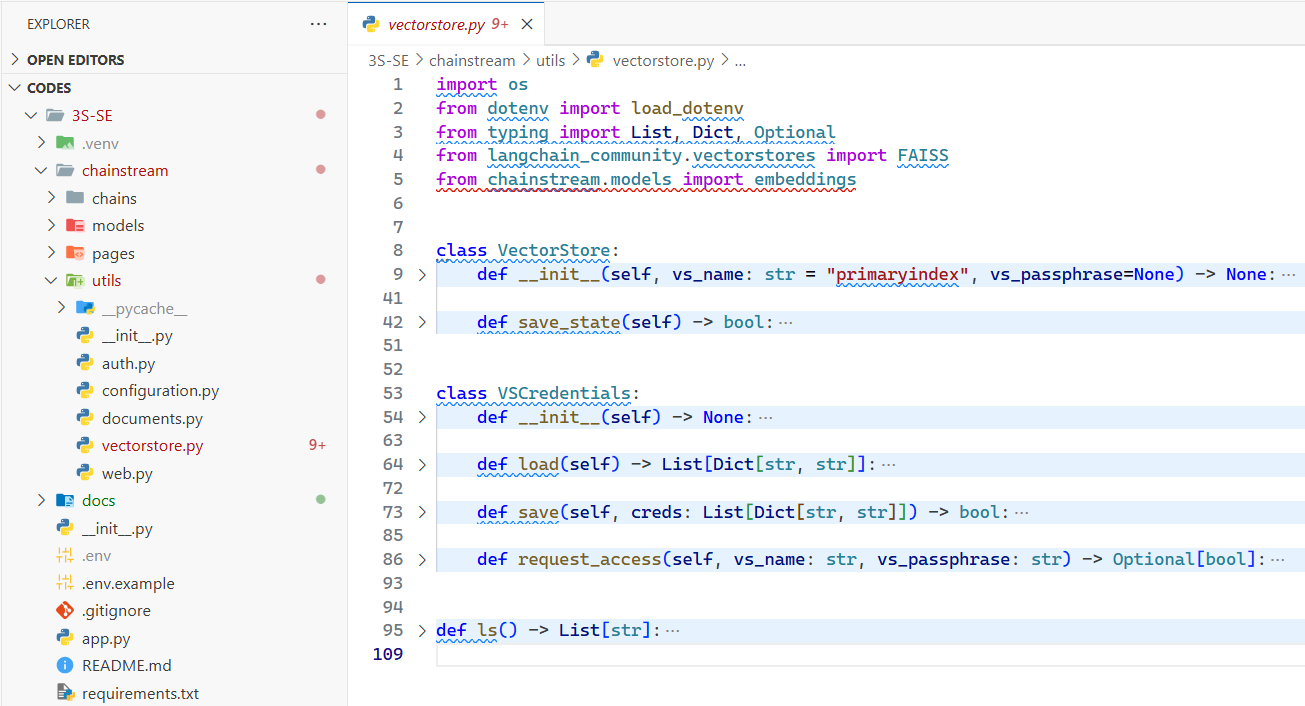
\includegraphics[width=\linewidth]{./figures/vectorstore-implementation.png}
    \caption{Vector Store implementation classes and methods}
\end{figure}
A vector store can be initialized with "vs\_name" alone, which gives the read access to its contents. To modify it however, one should provide it with a passphrase ("vs\_passphrase"), which would give users who have gained access the ability to load new content through the various data ingestion methods previously mentioned.
\begin{figure}[H]
    \centering
    
\includegraphics[width=.8\linewidth]{./figures/vectorstore-local-dir.png}
    \caption{Local Directory for storing vector stores.}
\end{figure}
The "creds.json" file store access credentials to the available vector stores, while other folders ("3S" and "SSS" in this example) holds the vector store's data.
\subsubsection{Chunking and Embedding}
A vector store initialization typically includes an embedding model initialization, which vectorizes the documents' chunks. For our case, as we chose to select a model from Hugging Face Hub ("all-mpnet-base-v2"), we need to ensure that the model is downloaded and stays up-to-date.
\begin{figure}[H]
    \centering
    \begin{subfigure}{0.45\textwidth}
        \centering
        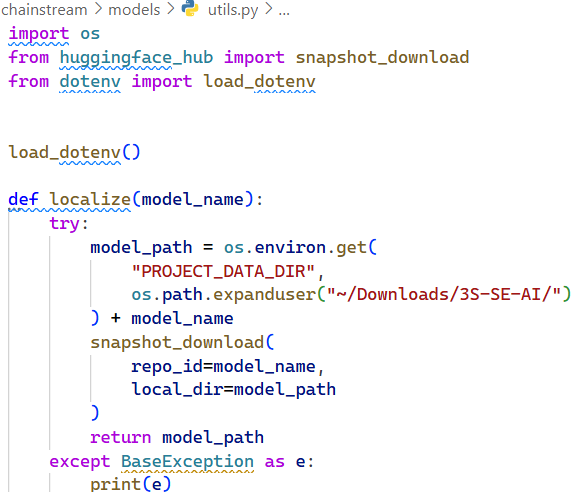
\includegraphics[width=\linewidth]{./figures/embedding-model-downloading.png}
        \caption{Downloading}
    \end{subfigure}
    \hfill
    \begin{subfigure}{0.45\textwidth}
        \centering
        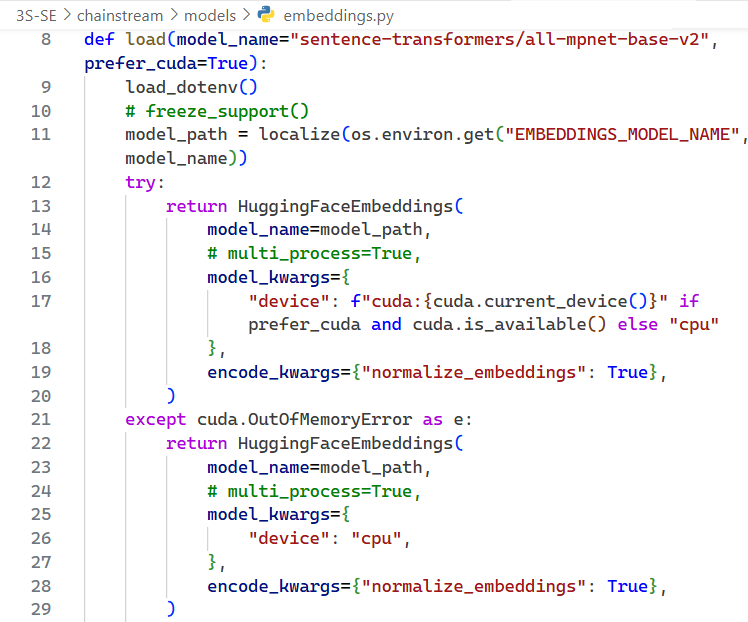
\includegraphics[width=\linewidth]{./figures/embedding-model-loading.png}
        \caption{Loading}
    \end{subfigure}
    \caption{Embedding Model Implementation}
\end{figure}
The "snapshot\_download" function imported from "huggingface\_hub" ensures that the latest version of the model is available locally and can be loaded, while the implemented `load` function leverages it by loading the model on the GPU and falls back to the CPU when needed.
\subsubsection{Retrieval and Similarity Search}
In some cases where the knowledge base does not contain relevant information to the user query, naive RAG would retrieve the passages with the highest similarity score, even if its contents are not pertinent to the question. This issue is addressed by only including documents whose scores attain a certain threshold, eliminating unnecessary passages thus reducing context size when prompting LLMs, and providing trustworthiness by informing the user when no content can be found rather than introducing hallucination in generated answers.\newline
Moreover, the context returned from the "base\_retriever" is further processed to compress and re-order its contents through a "Cross Encoder Reranker" based on its relevance to the queries, which ensures that its size can fit the diverse LLMs.
\begin{figure}[H]
    \centering
    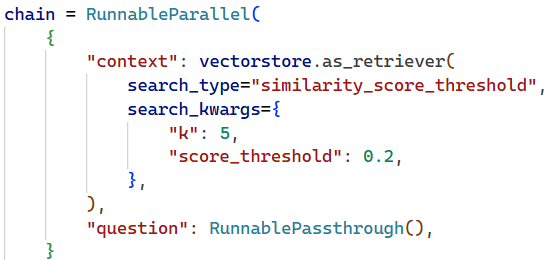
\includegraphics[width=.9\linewidth]{./figures/similarity_search_threshold.png}
    \caption{Similarity Search Tuning}
    \begin{flushleft}
        \small The "score\_threshold" parameter allows to set a value which only passages that have a higher score are passed to the LLM's context, while the "k" parameter controls the maximum number of documents.\newline The "base\_compressor" allows to introduce a passage re-ranking and compression tool (bge-reranker), which further reduces the size of the retrieved context without losing valuable information.
    \end{flushleft}
\end{figure}
\subsection{LLMs and Prompts}
As new products and cloud platforms are constantly emerging and changing rapidly, the models and tools (web searching APIs), which allow the LLMs to connect to external web searching APIs, were implemented in an extendible manner, where adding, removing or customizing LLMs and their behavior is an easy change in code. The following code snippet showcases the tool loading process when the environment is started.
\begin{figure}[H]
    \centering
    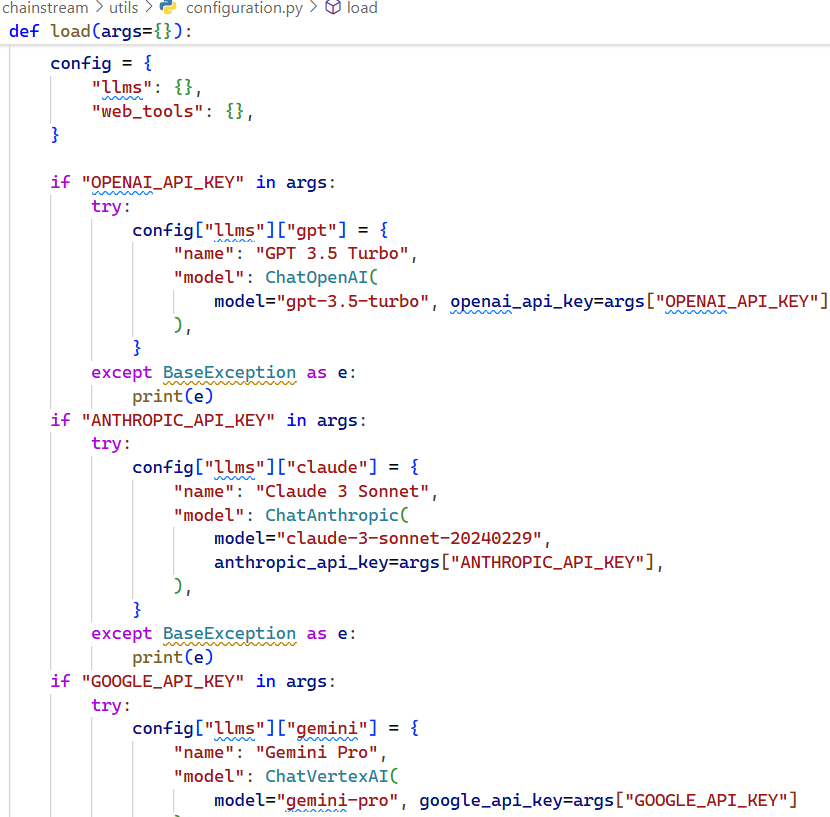
\includegraphics[width=.9\linewidth]{./figures/llms-implementation.png}
    \caption{Implementation of LLMs and Prompts, focusing on extensibility}
    \begin{flushleft}
        \small The lists of Large Language Models ("llms" key in the "config" variable) and tools ("web\_tools") grow dynamically when provided with valid API keys.
    \end{flushleft}
\end{figure}
The list is much longer than this illustration, still it is easy to figure out how to add other LLMs and APIs as needed.\newline
In addition to these APIs, this loading mechanism allows for flexible Prompt modification when different models require different prompts.
\begin{figure}[H]
    \centering
    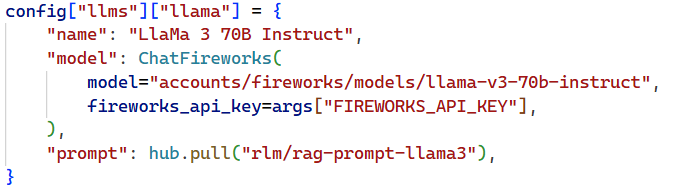
\includegraphics[width=\linewidth]{./figures/prompt-template-impl.png}
    \caption{Incorporating prompts into model definition.}
\end{figure}
This approach allows to define a custom prompt template suitable for a specific model (such as in our case of Llama 3) from within a unified source code file. In theory, the "prompt" field can hold any f-string format (a concept in Python used to interpolate variables dynamically into a string), but the \href{https://smith.langchain.com/hub}{LangChain Hub} provides many example prompts for different tasks.
\begin{figure}[H]
    \centering
    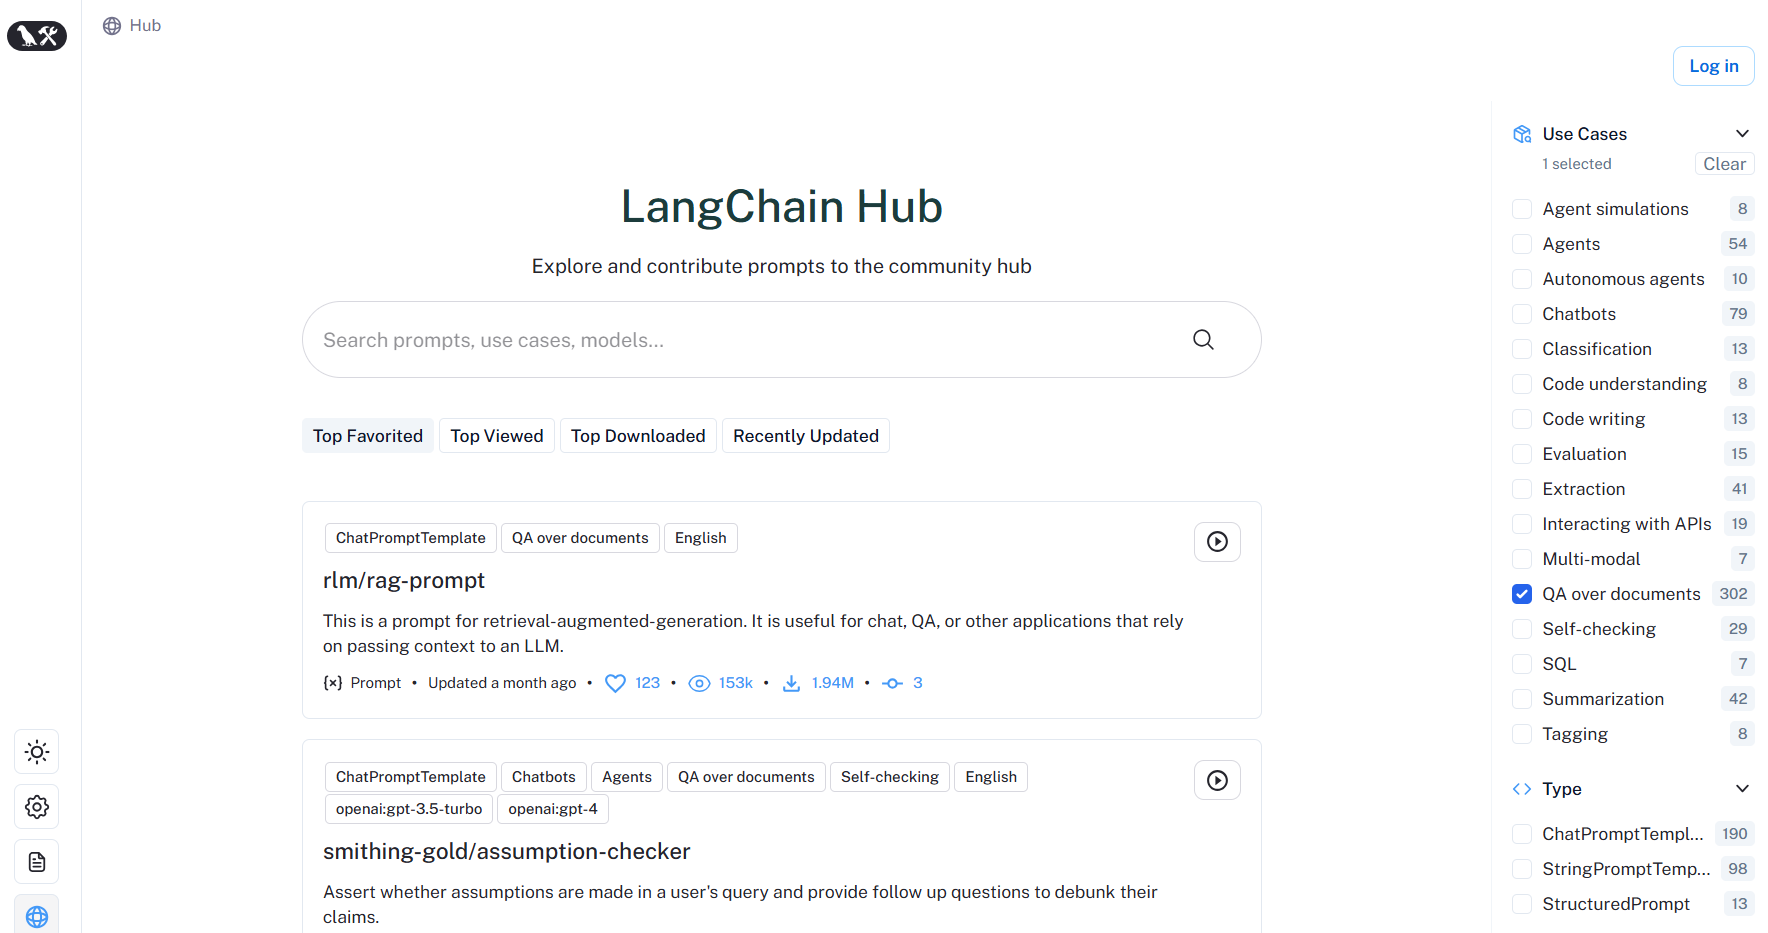
\includegraphics[width=\linewidth]{./figures/langchain-hub.png}
    \caption{LangChain Hub web interface.}
\end{figure}
This Hub allows to find ready-to-use prompt templates suitable for various LLMs for Retrieval-augmented generation purposes.\medskip\newline
The resulting list of implemented LLMs is as follows.
\begin{figure}[H]
    \begin{subfigure}{\textwidth}
        \centering
        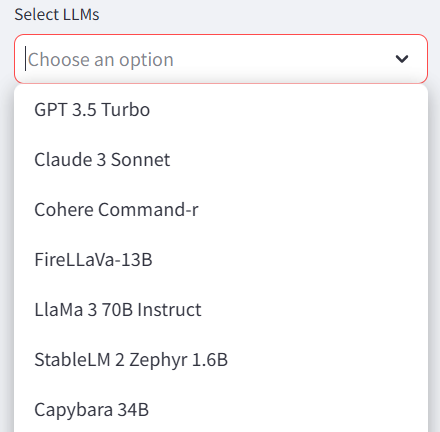
\includegraphics[width=.7\linewidth]{./figures/select-llms-p1.png}
    \end{subfigure}
    \begin{subfigure}{\textwidth}
        \centering
        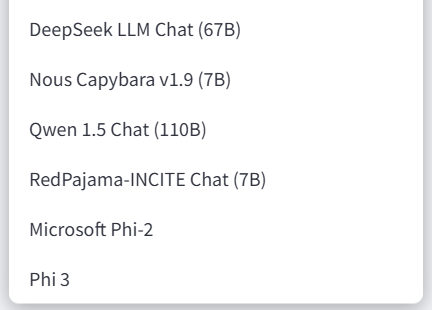
\includegraphics[width=.7\linewidth]{./figures/select-llms-p2.png}
    \end{subfigure}
    \caption{List of implemented LLMs}.
\end{figure}
\subsection{Evaluation and Ranking}
As multiple answer generations occur in parallel, it is essential to provide the better quality responses first. For this purpose, RAG-based metrics were implemented with the help of the Ragas library. It stands for Rag Assessment and provides various metrics to evaluate RAG pipeline performance.
\begin{figure}[H]
    \centering
    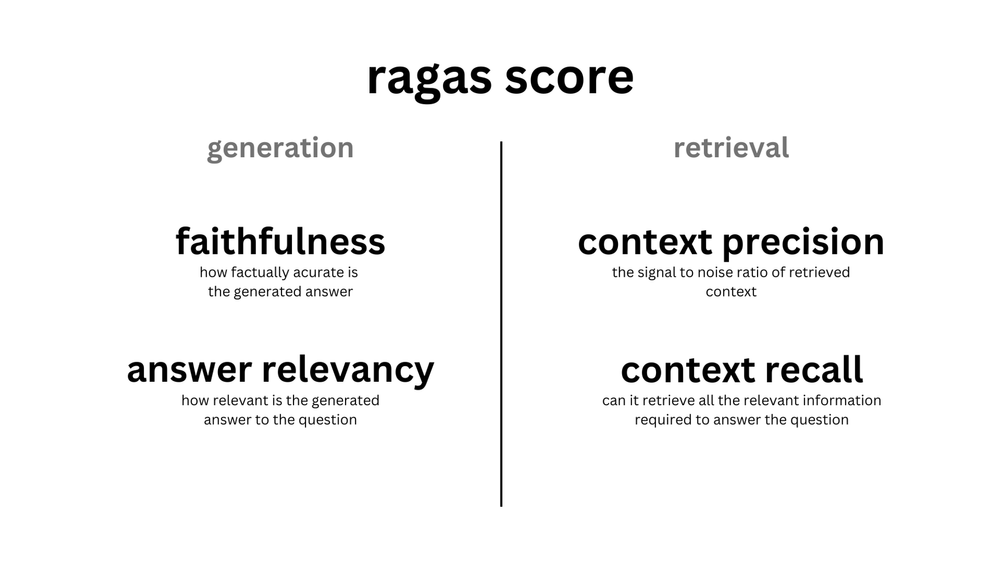
\includegraphics[width=\linewidth]{./figures/ragas-metrics.png}
    \caption{RAG pipeline evaluation metrics and description}
\end{figure}
When combined with the similarity score returned by the vector store when retrieving documents, this library allowed to assess the retrieval phase context relevancy and generation phase consistency against the given context and the prompt.
In addition to these metrics, a user-driven feedback was implemented and integrated into the ranking algorithm to assess the overall satisfaction over a specific Large Language Model.
\begin{figure}[H]
    \centering
    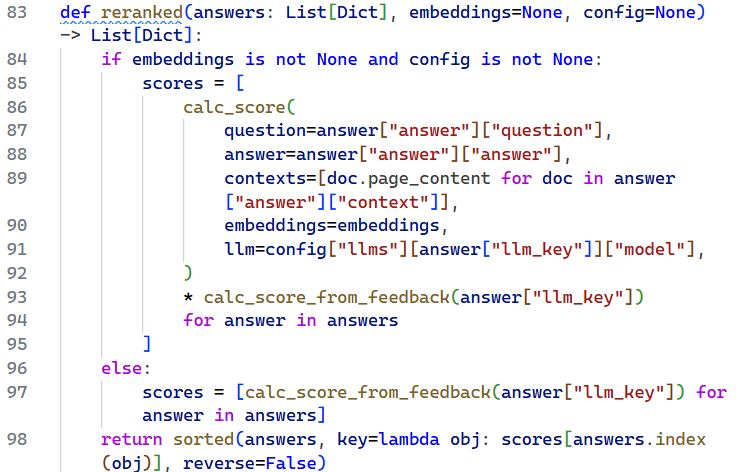
\includegraphics[width=\linewidth]{./figures/ranking-algo.png}
    \caption{Evaluation metrics for the ranking algorithm}
    \begin{flushleft}
        \small This function sorts the generated responses based on the evaluation scores measured for each model. It calculates the scores based on consistency of the generated answer against the given retrieved context and its relevancy to the query the model was prompted with, in addition to the feedback given by users. The formula to calculate the score is as follows :
        score = feedback score + faithfulness score + answer relevancy score
    \end{flushleft}
\end{figure}

\section{Conclusion}
This chapter has thoroughly detailed the development phase of the project. It has elaborated the technical choices of the components and their implementation.\newline
To evaluate our project design and implementation choices, we dedicate the next and final chapter to validate the results of the system by providing a comparison between our pipeline and a simple LLM generations, as the main goal of RAG is to build upon LLMs.

\chapter{Validation}

\section{Introduction}
This chapter is complementary to the previous one, and evaluates the refinement of the RAG pipeline to generated answers. In the following sections, we compare between the results from a simple call to a Large Language Model and the RAG pipeline, to observe the difference between the obtained results.

\section{Response without Retrieval-augmented Generation}
To obtain a response from a Large Language Model, it suffices to implement one from a cloud provider and prompt it with an example query, as shown in the following figure.
\begin{figure}[H]
    \centering
    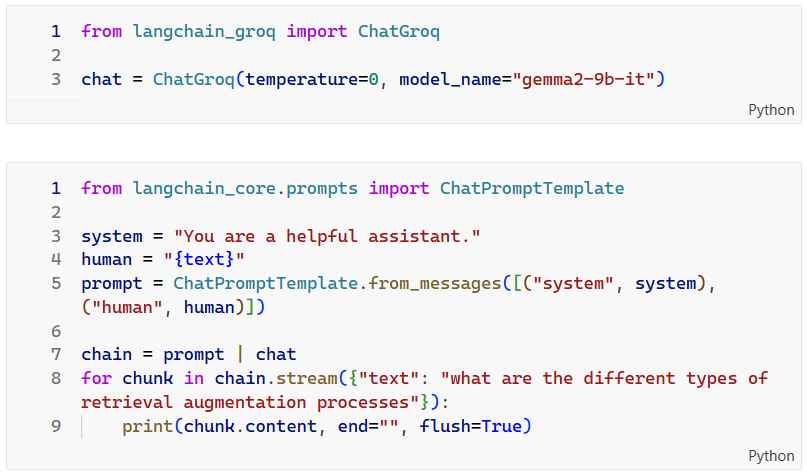
\includegraphics[width=\linewidth]{./figures/code-norag.png}
    \caption{Implementation of a question-answering LLM (No RAG)}
    \begin{flushleft}
        \small First, we start by initializing a chat model, Gemma-2 from GroqCloud, and instruct it to provide a helpful answer to a given question (what are the different types of retrieval augmentation processes).
    \end{flushleft}
\end{figure}
The response the chat model provided is demonstrated in the following illustration.
\begin{figure}[H]
    \centering
    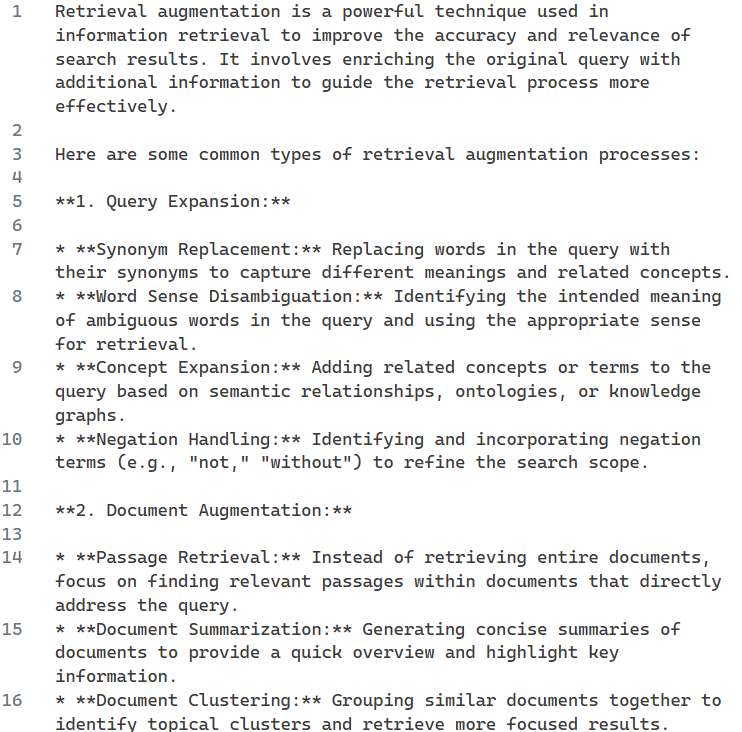
\includegraphics[width=\linewidth]{./figures/answer_norag.png}
    \caption{The response obtained from a LLM call directly}
\end{figure}
The example demonstrates the inconvenience of using an LLM when looking for a short and accurate response to a given query ("what are the different types of retrieval augmentation processes"). The generated answer is very long and clearly exhibits hallucination, as it is not accurate enough.\newline
The next section is about rectifying this inconvenience by implementing a RAG pipeline and providing relevant information from which the LLM base its response.

\section{Retrieval-augmented Generation Results}
\subsection{Data: Question and Answer}
We will need to load some data into the knowledge base. This information represents the ground truth on which we desire LLMs to base their answers.\newline
For this purpose, a \href{https://arxiv.org/abs/2312.10997}{PDF file from a research parper on Arxiv} will be uploaded as target data. Page 11 of this document contains the answer to our previous question, which we want to be automatically retrieved from the vector store.
\begin{figure}[H]
    \centering
    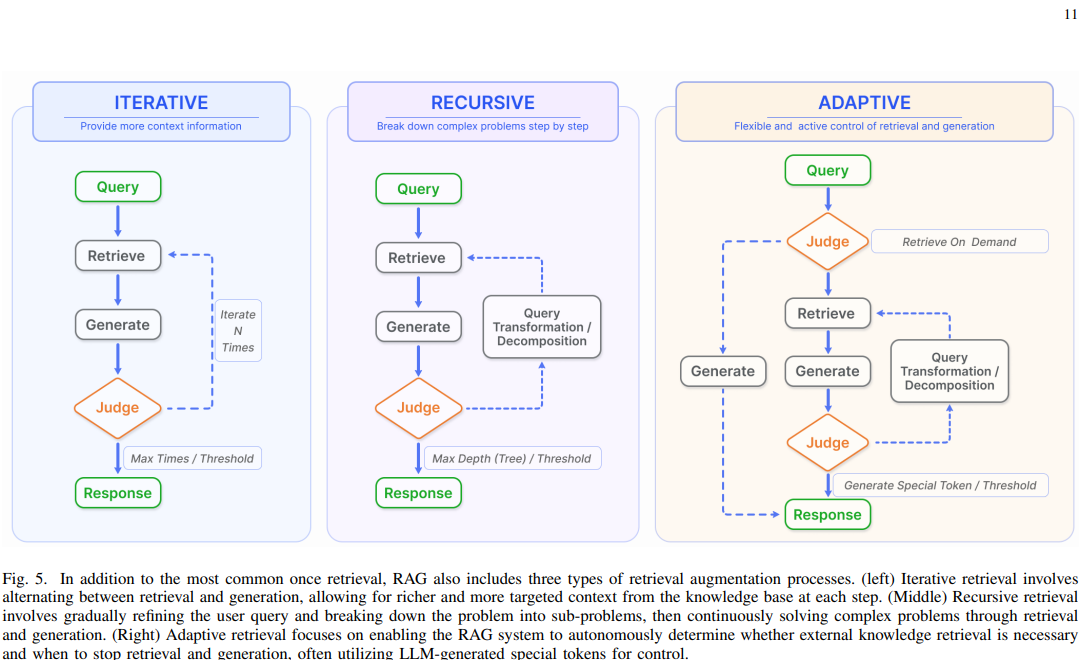
\includegraphics[width=\linewidth]{./figures/toberetrieved.png}
    \caption{The targeted context.}
    \begin{flushleft}
        \small This page from the PDF file contain clear answer to our question (3 types of retrieval augmentation processes: iterative, recursive, adaptive), explained in the caption.
    \end{flushleft}
\end{figure}
After having established a query to be asked to the model and its corresponding desired answer, we will now implement a simple RAG pipeline, similar to the one implemented in the system, with the same previous model (Gemma 2) to see the difference in generated answers.
\subsection{Knowledge Base initialization}
The first step is to load the PDF file into the knowledge base. For this purpose, we need to initialize a FAISS index with an embedding model (all-mpnet-base-v2), which will convert the information read from the file through PyMyPDFLoader to a numerical representation suitable for similarity search afterwards.
\begin{figure}[H]
    \centering
    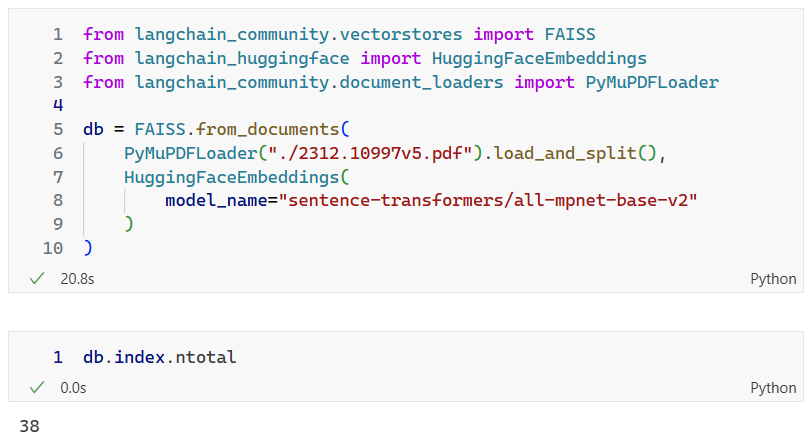
\includegraphics[width=\linewidth]{./figures/vectorstore_init.png}
    \caption{Vector Store initialization with data}
    \begin{flushleft}
        \small This sample vector store initialization included reading and loading the required PDF file from local storage, resulting in 38 chunks, which simplifies the process of retrieving and passing the most relevant chunks to the large language model later on.
    \end{flushleft}
\end{figure}
\subsection{Similarity Search dry run}
The following code imitates the retrieval phase in a complete RAG pipeline, providing an overview of the contents of the vector store and the results when some passages get retrieved.\newline
\begin{figure}[H]
    \centering
    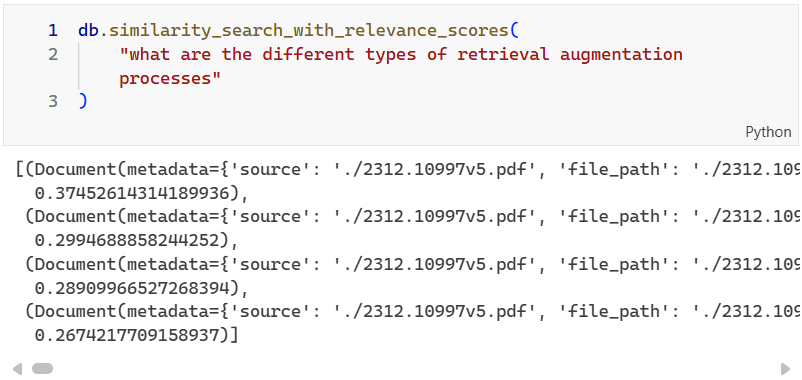
\includegraphics[width=\linewidth]{./figures/vectorstoresimilaritysearchwithscore_code.png}
    \caption{Retrieving relevant documents from the database}
    \begin{flushleft}
        \par The figure demonstrates a collapsed list of documents obtained from the database when applied to similarity search with the question "What are the different types of retrieval augmentation processes". The list is sorted by the cosine similarity score, and we can observe the passage we identified earlier as context in the third item.
    \end{flushleft}
\end{figure}
\begin{figure}[H]
    \centering
    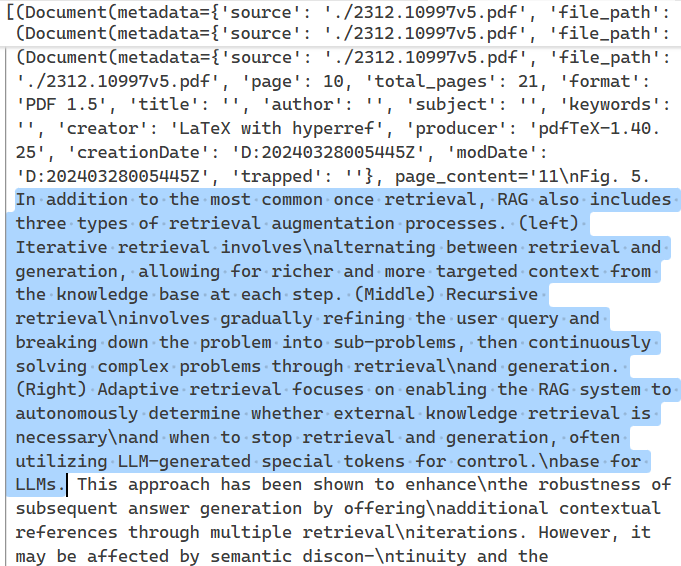
\includegraphics[width=\linewidth]{./figures/vectorstoresimilaritysearchwithscore_output.png}
    \caption{Output from similarity search}
    \begin{flushleft}
        \small The returned passages, as seen above, contain parsed text from the PDF file. As the vector store contain separate chunks, the result of running the previous code is a list containing document chunks, each with the textual content and some metadata that helps representing the whole documents through its chunks in a vector store. The highlighted text is the desired data that we want to pass to the LLM afterwards. This passage is returned 3rd on the list, with a score of 0.28.
    \end{flushleft}
\end{figure}
The results of retrieval, even though still optimizable (demonstrated later on in the answer sorting section), is satisfactory. Given a query, it is almost impossible to not retrieve the relevant passage outside the first 5 elements. This is because of the indexing strategy implemented in the vector store which allows to calculate the similarity between every chunk and the query to ensure most similar passages are retrieved effectively.\newline
These retrieved documents can now be integrated in a prompt and passed to the LLM to control the context of its generation process.
\subsection{Response with Retrieval-augmented Generation}
\begin{figure}[H]
    \centering
    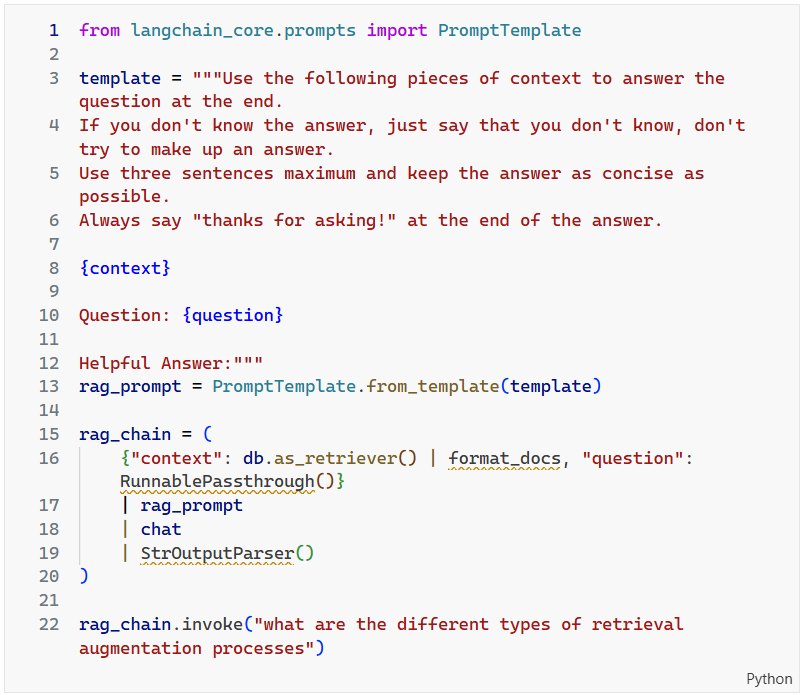
\includegraphics[width=.9\linewidth]{./figures/rag-code.png}
    \caption{Initialization of a simple RAG pipeline for testing}
    \begin{flushleft}
        \small The steps to initialize the RAG pipeline are: 1. set the prompt to support passing the context (retrieved documents) and question, along with instructing the model to only base its answer on the given context, 2. reconstructing the prompt by filling the variables (retrieving and formatting the context and the question), 3. passing the constructed prompt to the LLM (chat), 4. and finally transforming the LLM's response into a human readable format.
    \end{flushleft}
\end{figure}
Executing the previous code resulted in the desired output.
\begin{figure}[H]
    \centering
    
\includegraphics[width=\linewidth]{./figures/rag-answer.png}
    \caption{A simple RAG pipeline's generated answer}
\end{figure}
The response demonstrates how effective was the pipeline from transforming a long irrelevant answer into a very accurate and direct one.

\section{Answer Sorting}
The sorting algorithm allows for better answers to be more accessible by placing them at the bottom of less accurate ones (in our case where multiple LLMs attempt to generate the most suitable response given the same context).
To showcase how it affects the results page, here is a comparison between the positioning of generated answers from four different models (Claude 3.5 Sonnet, Command R+, Gemma-2 and Llama-3), using the previous example's question and data while employing the system's advanced RAG pipeline with its additional subprocess and phases.
\begin{figure}[H]
    \centering
    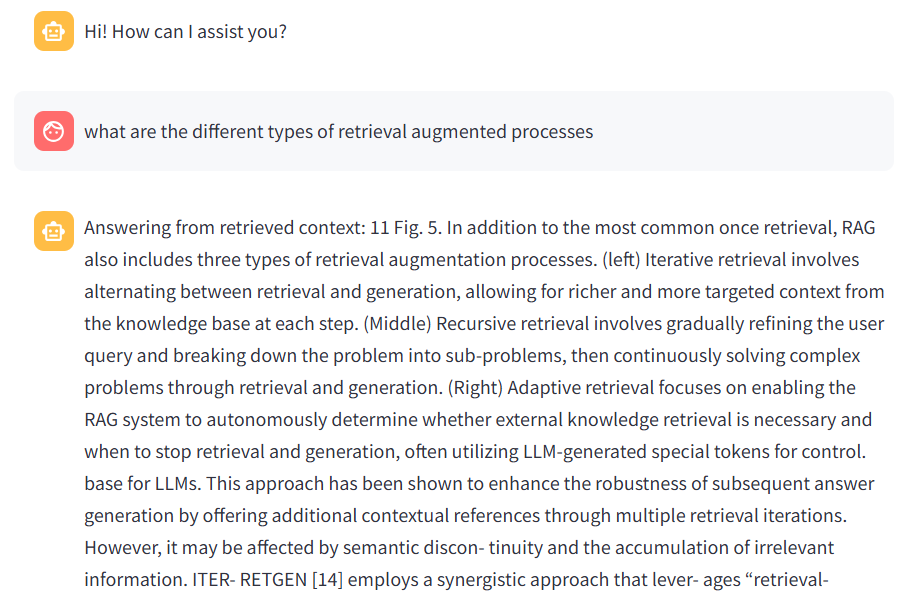
\includegraphics[width=\linewidth]{./figures/app-question.png}
    \caption{Prompting and retrieving context from the input question}
    \begin{flushleft}
        We can remark the effect of the re-ranking algorithm employed in the RAG pipeline, which prioritized the passage we identified in the first part of the "RAG results" previously.
    \end{flushleft}
\end{figure}
After the context gets retrieved from the selected vector stores, the LLMs generate answers based on its contents as shown below.
\begin{figure}[H]
    \centering
    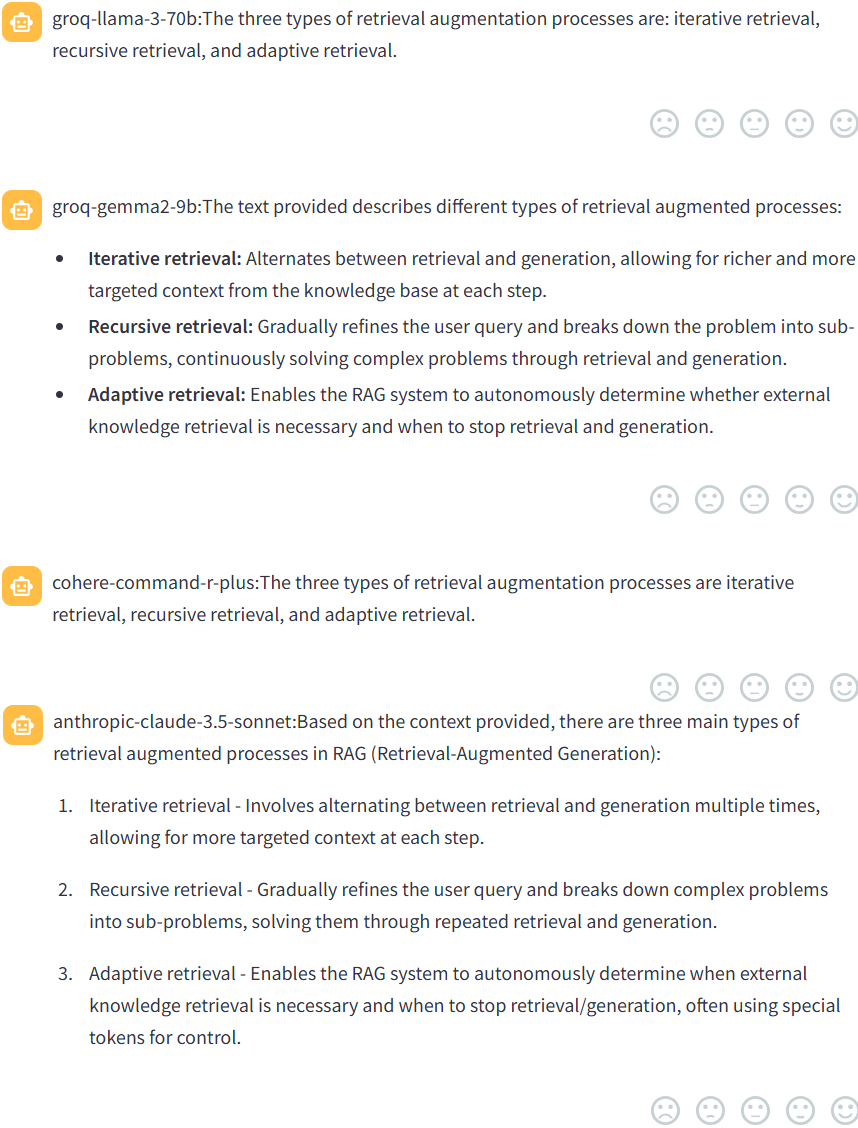
\includegraphics[width=.8\linewidth]{./figures/app-answers.png}
    \caption{Generated answers: not sorted}
\end{figure}
We can observe that the generated answers have clear differences. Some models perform better than others in certain cases, and this behavior alternates, meaning it is impossible to determine the best models for every use case. For this example, all the models generated relevant answers, but Claude and Gemma provided further accurate details. The results, however, are not sorted in any order, except the order of which the user has selected their preferred LLMs. It is possible that the more accurate responses get shadowed by less relevant ones (as the case with the Gemma-2 response in this example). Our goal for this app is to allow users to select the LLMs they prefer, while prioritizing better answers first automatically, which can be achieved by checking an option in the web interface to toggle the sorting algorithm.\newline
The following figure demonstrates the ranking of the previous answers to prioritize better quality results.\newline
The Gemma-2 and Claude-3.5 models performed better than the other models, providing more information extracted from the retrieved context, while Llama-3 and Command R+ did not use the available information from the context and generated more succinct answers.\newline
\begin{figure}[H]
    \centering
    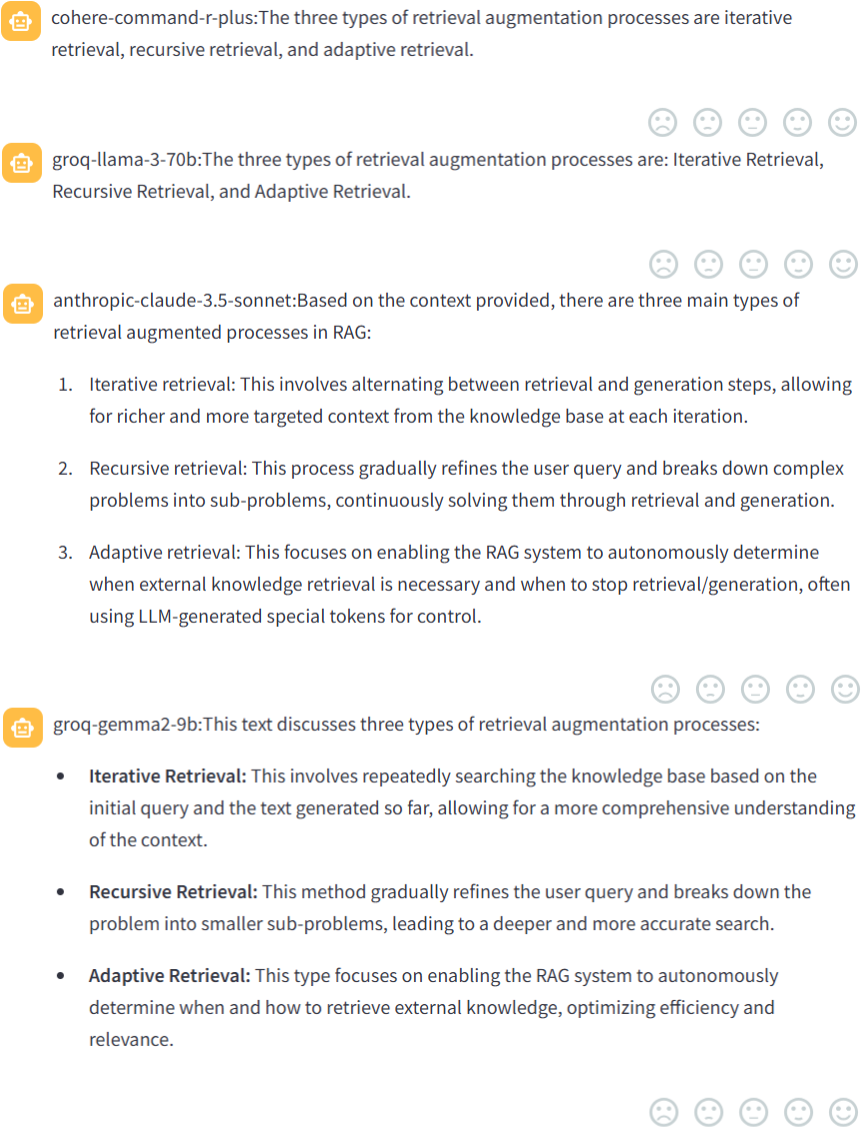
\includegraphics[width=\linewidth]{./figures/app-answers-sorted.png}
    \caption{Generated answers: sorted}
    \begin{flushleft}
        The ranking algorithm employed metrics specifically designed to evaluate RAG processes, measuring the consistency of the generated response against the given context, and assessing its pertinence to the original prompt.
    \end{flushleft}
\end{figure}

\section{Conclusion}
In conclusion, this project has demonstrated the efficacy of implementing and orchestrating a RAG pipeline to provide accurate and factual responses from a knowledge base. The employed retrieval phase methods can be used standalone to provide comparable results, but with the addition of a generation phase, we can leverage the NLP capabilities of LLMs to tune the responses to user queries and enrich results with valuable insights.

\chapter*{General Conclusion}
\addcontentsline{toc}{chapter}{General Conclusion}
\hspace{1cm}This project has resulted in the successful design and implementation of a RAG pipeline. By effectively combining the strengths of LLMs and vector stores, the tool demonstrates the potential to revolutionize how the organization manage and access their information assets.\bigskip

The RAG pipeline architecture, incorporating data ingestion, preprocessing, embedding generation, vector store indexing, and query processing, has been meticulously designed to ensure optimal performance and accuracy. The employed LLMs, with their advanced language understanding and generation capabilities, have proven to be instrumental in extracting valuable insights from the data. The vector store, efficiently storing and retrieving embeddings, has significantly enhanced the search capabilities of the tool by retrieving relevant contexts.\bigskip

While the project has achieved its primary objectives, there are opportunities for further exploration and improvement. These include employing local Large Language Models in order to make it possible to fine-tune them based on company data, or to employ Reinforcement Learning from Human Feedback techniques by allowing user interaction with generated responses, or to explore other retrieval techniques, like leveraging some type of LLMs (document-answering task models from Hugging Face Models Hub) which can give more accurate retrieval results. Additionally, a new approach of RAG, called GraphRAG, is currently being developed by Microsoft, which allows to build a graph knowledge base that make the LLMs more capable to extract and understand the relationships between entities from the knowledge base.\bigskip

In conclusion, the implemented RAG-based enterprise knowledge searching tool represents a significant step forward in harnessing the power of AI for information retrieval. It has the potential to streamline workflows, improve decision-making, and unlock new opportunities for the company.

\begin{thebibliography}{9}
    \bibitem{ragforllmsasurvey}
    \href{https://arxiv.org/html/2312.10997v5}{Retrieval-Augmented Generation for Large Language Models: A Survey}

    \bibitem{scrum}
    \href{https://www.scrum.org/resources/what-scrum-module}{What is Scrum (scrum.org)}

    \bibitem{faissess}
    \href{https://engineering.fb.com/2017/03/29/data-infrastructure/faiss-a-library-for-efficient-similarity-search/}{Faiss: A library for efficient similarity search}

    \bibitem{langchainvectorstore}
    \href{https://python.langchain.com/v0.1/docs/modules/data_connection/vectorstores/}{LangChain Documentation}

    \bibitem{weaviateindexing}
    \href{https://weaviate.io/developers/weaviate/concepts/vector-index}{Vector Indexing | Weaviate}

    \bibitem{zsimilaritymetrics}
    \href{https://zilliz.com/blog/similarity-metrics-for-vector-search}{Similarity Metrics for Vector Search - Zilliz Blog}

    \bibitem{bivscrossencoders}
    \href{https://www.sbert.net/examples/applications/cross-encoder/README.html}{Cross-Encoders - Sentence Transformers documentation}

    \bibitem{aidomainsrel}
    \href{https://blog.miarec.com/contact-centers-ai-definition}{Understand AI, ML \& Co in Contact Centers: Definitions \& Explanations - miarec}

    \bibitem{transformersarch}
    \href{https://arxiv.org/abs/2002.04745}{On Layer Normalization in the Transformer Architecture}

    \bibitem{prompts}
    \href{https://www.oajaiml.com/uploads/archivepdf/63501191.pdf}{A Study on the Implementation of Generative AI Services Using an Enterprise Data-Based LLM Application Architecture}

    \bibitem{langchainmodules}
    \href{https://python.langchain.com/v0.1/docs/modules/}{LangChain Documentation}

    \bibitem{hfmhdocs}
    \href{https://huggingface.co/docs/hub/models}{Hugging Face Models Hub documentation}

    \bibitem{hfmodels}
    \href{https://huggingface.co/models}{Models - Hugging Face}

    \bibitem{langchainllmintegrations}
    \href{https://python.langchain.com/v0.1/docs/integrations/llms/}{Langchain Documentation - LLMs}

    \bibitem{togetheraipg}
    \href{https://api.together.ai/playground}{TogetherAI Playground service}

    \bibitem{sbertsentencetrans}
    \href{https://sbert.net/docs/sentence_transformer/pretrained_models.html}{Pretrained Models - Sentence Transformers documentation}
\end{thebibliography}

\includepdf[pages={2}]{./pdfs/Page Garde Rapport Stage(Ang) 2.pdf}

\end{document}